
\documentclass[12pt]{article}
\usepackage{cite}
\usepackage{graphicx}
\usepackage{float}
\usepackage{subfig}
\usepackage[a4paper]{geometry}
\geometry{hscale=0.85,vscale=0.85,centering}

\def\xcolorversion{2.00}
\def\xkeyvalversion{1.8}
\usepackage[version=0.96]{pgf}
\usepackage{tikz}
\usetikzlibrary{arrows,shapes,snakes,automata,backgrounds,petri}


\usepackage{algpseudocode} 
\usepackage{algorithm}


\hyphenation{op-tical net-works semi-conduc-tor}

\usepackage{titling}

% Make a clickable table of content
\usepackage{hyperref}
\hypersetup{
	colorlinks,
	citecolor=black,
	filecolor=black,
	linkcolor=black,
	urlcolor=black
}

% Put the bibliography in the table of contents
\usepackage[nottoc,notlof,notlot]{tocbibind}    

% For multirow tables
\usepackage{multirow}


\setlength{\droptitle}{-4em}   % This is your set screw

\title{Robotic models of learning and development \\of speech and tool use.}

\author{S\'ebastien Forestier}





\begin{document}


\maketitle
\thispagestyle{empty}
%\vspace{1em}
%\textbf{Supervisor:} Pierre-Yves Oudeyer


\vspace{2em}
%\paragraph{Abstract}

	Documentation and roadmap of my Master's internship and the beginning of my PhD thesis.

%

\vspace{2em}

	\begin{figure}[H] 
		\centering 
		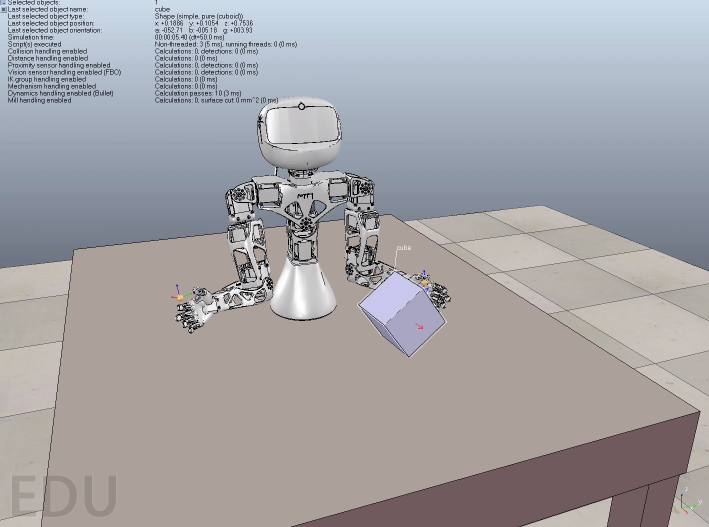
\includegraphics[height=10cm]{./include/torso.png}
	\end{figure}  	


\newpage
\tableofcontents
\newpage


\section{Introduction}

	\paragraph{}
	During their first years of life, infants progressively learn to make complex arm gestures and finger movements to interact with the objects of the environment.
	At the same time, they also learn to produce physical effects on the world with another mean.
	They discover that some of their
	vocalizations can be used as tools to influence their social peers, as through the action of these social peers they are able to produce physical effects.
	To do so they learn how to use their vocal tract composed of many complex actuators from the larynx to the lips.
	An important scientific question is how these influences are discovered and by which mechanisms the corresponding abilities are developed.

	\paragraph{}%
	Recent work in computational modeling has shown how mechanisms of active curiosity-driven learning, combined with imitation learning, 
	could progressively self-organize
	developmental stages of increasing complexity in vocal skills.
	These developmental stages share many properties with
	the vocal development of infants in the first 6 months of life \cite{moulin-frier_self-organization_2014}.
	
	\paragraph{}
	Like in other computational models of vocal development \cite{guenther2006neural, howard2011modeling, warlaumont2013prespeech}, 
	the vocal agents in the model of Moulin-Frier et al. do
	not associate sounds to meaning, and do not link vocal production to other forms of action.	
	In other models of language acquisition, one assumes that vocal production is mastered, 
	and	hand code the meta-knowledge that sound should be associated to referents or actions \cite{mangin2012learning}.
	But understanding what kind of mechanisms can explain the smooth transition between the learning of vocal sound
	production and their use as tools to affect the world is still largely an open question.

	\paragraph{}
	In this work, we will extend models of curiosity-driven goal babbling and
	their interaction with social interaction presented in \cite{moulin-frier_self-organization_2014} so as to make
	steps towards addressing this question. 	
	In particular, we will integrate
	additional mechanisms to handle task and action
	spaces where the task spaces initially given to the robot can be encapsulated
	as primitive actions to affect newly learned task spaces.
	
	\paragraph{}	
	We will first develop simple extensions of the SAGG-RIAC architecture with different sensorimotor models that can be learned in a hierarchical manner.	
	A sensorimotor model is defined as first a task spaces (or sensori space) where tasks (or sensori states to be reached) can be set by a teacher, 
	or self-generated by the learner and also a motor space to be used to solve those tasks.	
	A sensorimotor model is learned well enough when the learner knows how to solve the tasks (or reach sensori goals) for which it has the means to.
	Then, in an action to solve a new task, a new model can reuse that previous model by giving it a sub-task that will be useful to solve the current one.
	We are here describing a hierarchy of models that the agent can learn and extend with new ones.
	
	\paragraph{}
	Given a simple hierarchy of 2 models, one reusing the other, a straightforward learning mechanism will be to explore the first model 
	and after some time, to explore the second one. 
	We will also study other mechanisms to handle this hierarchy of sensorimotor models that all need to be explored with an certain amount of trials that 
	the agent could estimate.	
	
	\paragraph{}
	In order to evaluate the hierarchical learning mechanisms, we will describe a first task for which a simple hierarchy of 2 sensorimotor models
	with the second reusing the first can be used to learn the task.
	A simulated robot arm will have to explore its motor space in order to understand how to push an object to different locations. 
	The robot will first explore how to make movements with its hand and then use this skill to explore the task of pushing an object.		
	The simulated environment having a high variability due to collisions' unstability, that makes comparisons of architectures difficult.	
	We will thus also implement a more simple environment composed of a simple geometric arm moving in 2 dimensions.
	Then, more complex hierarchies will be tested in an environment with the simple arm where a sequence of 2 movements has combinatorial 
	consequences on the sensors. 
	
	\paragraph{}
	Measuring exploration or learning is not generally equivalent. 
	Exploration is a measure of how well the agent has found diverse outcomes in its task space. 
	It makes no assumptions about the interest of exploring given regions of the task space from the viewpoint of the engineer, 
	neither if we want the robot to learn specific tasks or if we know that certain tasks will be more useful later for the robot.
	However, in unstable parts of the sensorimotor environment, the exploration measured makes no sense for the robot as it might not have the competence to 
	reach again that goal.
	For instance when a robot is trying to throw a ball to given position on a table, 
	even if the robot tries the same motor command, it might never reach again a reached position due to the variability in the generated arm movement, and 
	the collision between the arm and the ball.
	On the other hand, learning measures the competence of the robot on some tasks: how well the robot reaches a set of user-defined 
	goals of the task space. The agent is evaluated on some tasks even if it did not know that it 
	would be evaluated on those tasks. 
	As the agent self-generates goals in the task space, it might not yet have explored that evaluated part of the environment, or in another run, have explored
	it very early, so it is hard to interpret this competence as a general progress.
	We will thus define an intermediate measure that will evaluate how well competent is the robot on the explored part of the task space.
	
	\paragraph{}
	Then, in order to assess a possible development of language seen as a tool to produce physical effects on an environment, 
	we will develop a multi-modal environment composed of the DIVA vocal synthesizer \cite{guenther2006neural} and the previous 2D arm, in which combinations 
	of sounds and arm movements make combinatorial changes in the environment.
	
	\paragraph{}
	In the firsts learning algorithms developed, the hierarchy of models to learn is given to the agent as if it already knew the combinations of actions
	to explore in order to learn the successive tasks.
	This is a strong hypothesis as infants have first to discover what types of actions to combine to get a specific outcome.
	For instance, the discovery that pushing on the knees and on the arms with certain coordination for a 6-month-old baby allow to move with an interesting high speed, but it does not need to be taught by parents.
	We will then develop an algorithm to autonomously complexify the sensorimotor contingencies learned by reusing the previously learned actions, with no
	predefined hierarchy of sensorimotor models.
	In this work we did not have time to assess those learning architectures but that will be done in future experiments.
	
	%We will describe an algorithm that integrates the different interest model of higher models in the hierarchy to guide the exploration of the current model.
	
	\paragraph{}
	Finally, we will derive a way to integrate those hierarchical learning architectures with social interactive learning 
	from the SGIM-ACTS learning architecture \cite{nguyen2012}. 
	Different implementations will be developed, that could allow imitation of teachers and more generally social guidance in our models.
	The evaluations of those social learning algorithms remains to be done.
	
	\paragraph{}
	In the next section, related work will be presented on curiosity-driven learning, models of language acquisition, hierarchical representation of actions
	and social interaction.
	In Section 3, the methods of the experiments will be explained and we will present the details of the algorithms.
	In Section 4, the results of the conducted simulations will be presented, and a general discussion will be developed in Section 5.

	%
%
	
\section{Related work}

	\subsection{Curiosity-driven exploration and developmental trajectories}
				
		
		\paragraph{}
		Active curiosity-driven learning is a paradigm in which the robot or learning agent chooses itself what to explore or learn in its environment, 
		based on some sort of internal model of its progress in the task of exploring or learning \cite{cangelosi2010integration}. 
		With an intrinsic motivation to explore and learn in interesting situations, situations where the agent is progressing the most, the expected future progress is thus maximized.
		The agent does not necessarily know exactly what engineers are expecting from it, or on what task it should measure its own progress, 
		but general principles permit to define what is an interesting situation. 
		If the agent builds an internal model of its sensorimotor contingencies (e.g. What happen if I push that button ?), then it can monitor the accuracy of its sensorimotor model
		by experimenting with its environment, and compute the progress of its sensorimotor model, that will lead it to bias its experiments in those regions of the sensorimotor 
		model that have shown a high prediction progress.
		
		\paragraph{}
		These ideas of curiosity-driven learning have a grounding in infants psychological experimentation \cite{forestierworkshop} that show that infants are seeking, by play,
		situations of intermediate novelty: situations neither too novel, neither fully understood.
		For instance, in order to understand how infants learn about the statistical properties of their sensory environment, 
		Kidd and collaborators \cite{kidd} have tested 
		how 8-month-old infants' attention to their environment is modulated by its statistical complexity.			
		They presented 3 objects popping out of their respective boxes, in a sequence of varying complexity, 
		as measured by its information content or surprise: the negative log probability of an object popping out of a given box.
		The measure of infants' attention is related to the time after which they look away from the object, given by eye-tracking tools.						
		They show that infants have a Goldilocks preference: a preference for sequences neither too simple nor too complex.				
		The explanation of this effect is that this preference gives infants a useful rate of sensory information 
		and to avoid wasting cognitive resources on too complex stimuli.		
		This is defined also in the "Flow" theory \cite{flow} defining a state of pleasure obtained when engaged in activities challenging enough but not too much.
		
		\paragraph{}%
		In order to model information seeking mechanisms and curiosity-driven learning suggested by behavioral experiments in humans and animals,
		Pierre-Yves Oudeyer uses an embedded setup with developmental robots. Those robots are learning in an open-ended manner: they are not defined to solve any task but rather are designed 
		to be able to adapt to any unpredicted environment.		
		%
		The authors developed computational architectures to handle this curiosity driven learning: including the IAC \cite{oudeyer_intrinsic_2007} 
		and SAGG-RIAC \cite{baranes2010intrinsically} architectures.
		Here an intrinsic motivation to discover the sensorimotor environment is defined as a measure of prediction progress in the motor space (IAC) 
		or competence-progress in the sensory space (SAGG-RIAC).
		%
		The SAGG-RIAC architecture keeps a predictive model of the competence progress of the robot in different explored parts of the sensory space.
		To measure its own competence, the robot is self-generating goals to reach in the sensory space, and see how close to the goal it manages to go.
		The exploration is then biased towards parts of the space which give the highest competence progress, this mechanism ensuring a useful exploration in a space of high dimensionality where random exploration would not enable any learning. 			
		Implementations of these ideas include the Playground Experiment \cite{oudeyer_intrinsic_2007} and self-organization of vocalizations \cite{moulin-frier_self-organization_2014}.
		
		\paragraph{}%
		In the Playground Experiment, a quadruped robot is placed in an infant play mat, with a responding robot peer next to it. 
		The robot has to learn how to use its motor primitives to interact with its environment (IAC architecture). 
		They observe the self-organization of developmental	trajectories: in different runs with the same parameters, the robot explores objects and actions with 
		different orders.
		
		\paragraph{}%
		In the self-organization of vocalizations experiments, a simulated agent has to understand how to use a vocal synthesizer with the help of humans' phonetic items. The SAGG-RIAC architecture can generate phonetic goals to reach with the simulated vocal tract, in parts of the sensory space where competence progress is high, or try to imitate humans' phonetic items, choosing the strategy that again shows the best competence progress.
		They conclude that developmental trajectories of increasing complexity are emerging, with regularity and diversity.
		The diversity comes from different mechanisms: random generation in the algorithms, variability in the environment, and the multiples attractors
		of the learning dynamic system.
				
		\paragraph{}%
		These developmental trajectories are similar to what can be observed during child development, which is an evidence toward
		a general purpose curiosity-driven system in infants' learning \cite{oudeyer2014evolution}. 
		A behavioral and cognitive epigenesis could develop and complexify behavioral and 
		cognitive phenomena by the interaction with the environment. Hence communication skills could be the result of curiosity-driven exploration.
		Thus curiosity-driven learning, as an exaptation mechanism, could develop skills useless at the moment but which can turn to be recruited 
		later for more complex unforeseen competences.			
		This idea leads them to an evolutionary perspective saying that an intrinsic motivation for learning for itself, could have become at some evolutionary point a more efficient mechanism than one for developing specific genetically encoded skills to survive and reproduce \cite{oudeyer2014evolution}.
		
		\paragraph{}
		In our hierarchical implementations, even if the sensorimotor models will be part of a hierarchy of models, 
		each of them will be explored using the SAGG-RIAC algorithm. 
		Another computational layer will have to choose which model to explore based on their learning progress.

	%
	
	\subsection{Models of language acquisition}
	
		\paragraph{}
		In some models of language acquisition, the produced sounds are not related to actions the agent or the caregiver 
		could make on the objects of the environment.
		The DIVA model (Directions Into Velocities of Articulators, \cite{guenther2006neural}) 
		is a neural network that simulates the cortical interactions to produce
		syllables, that provides an account of different production phenomena, from speaking skill acquisition to coarticulations.	
		%
		The Elija model \cite{howard2011modeling} also uses an articulatory synthesizer to pronounce sounds. 
		It first gets a reward for exploration of its vocal outputs, and then 
		is interacting with a modeled caregiver that imitates its sounds like a mother would do: 
		either mimicking the infant's sounds or rather providing an intermediate 
		sound between the infant's one and the adult one. 
		The model learns the associations between its vocal commands and the response of the caregiver.
		The agent can thus learn the name of objects by trying to reproduce caregiver's utterances.		
		%
		In a self-organizing map neural network model of motor prespeech production \cite{warlaumont2013prespeech}, experiments
		show that a reinforcement based on the similarity of the model's output sounds 
		with a given set of vowels can bias the post-learning model's babbling sounds
		towards that reinforced set of vowels.
		
		\paragraph{}
		In other models of language acquisition, one assumes that vocal production is mastered, and
		hand code the meta-knowledge that sound should be associated to referents or actions.
		For instance, the model from Mangin et al. \cite{mangin2012learning} gets as input dance-like combinations of human movement primitives plus ambiguous 
		labels associated to these movements.
		Using Non-negative Matrix Factorization \cite{paatero1994positive}, the model learns to recognize the movement primitives common to them, 
		and when given new combinations, is able to produce a good set of 
		labels to describe the combination.

		\paragraph{}
		We rather suppose that the agent has to autonomously learn that vocal sounds can be used, as tools, to affect the environment.
		

	%
	
	\subsection{Hierarchical representation of actions}
	
		\paragraph{}
		The study of the control of manipulation actions in humans has revealed a modular representation of actions 
		either in the cerebral cortex and in the spinal 
		cord with compositionality: an infinite number of movements can be expressed through combination of simple primitives, 
		and generalization: certain neurons (higher 
		in the hierarchy) can represent actions independently of the effectors used \cite{cangelosi2010integration}.
		
		\paragraph{}
		The same idea holds for language expressiveness which is based on syntactic hierarchical combinations 
		on a vocabulary, that open infinite semantic possibilities. 
		Greenfield has also argued that this parallel between manipulation and language compositionality can be found in the human ontegenic development
		with combinatorial steps for manipulation and syntax acquired approximately at the same period and in the same order \cite{green}. 
		Also, the author explains that the development of the neural substrates for language and tool use could be an ontogenic homology as first of all
		the same neural computations for hierarchical combinations and their semantics should take place for both modalities, and furthermore 
		experiments with Broca's and Wernicke's aphasics show that hierarchical organization for language and manipulation is linked. 
		Broca's aphasics, who have less syntactic organization of speech were shown to also have problems of representation of the hierarchical organization
		of constructions with blocks, whereas Wernicke's aphasics, whose syntax is normal but speech semantics is impaired, succeed in representing such objects 
		hierarchies. 
		
		\paragraph{}
		Functional MRI experiments by Higuchi et al. have shown that the human's neural substrates for tool use and language is indeed shared in 
		the dorsal BA44 Broca's area \cite{higuchi}, which gives evidence for the similar neural computations used. 
		They furthermore argue that these results supports the hypothesis that tool use have appeared first in primate evolution in F5 area,
		and then the language has developed in humans reusing part of tool use and manipulation neural substrates in human's Broca area, homolog of primate's F5.
	

		\paragraph{}
		Like a developing child, a developmental robot will have to incrementally explore skills that add up to the hierarchy of previously learned skills 
		throughout its life, with a constraint being the cost and time of experimentation. 
		We will seek to define curiosity-driven hierarchical learning architectures 
		that could reuse the sensorimotor contingencies previously learned and to combine them 
		to explore more efficiently new complex sensorimotor models. 
		
		\paragraph{}
		Different computational models have the possibility to learn skill hierarchies. 
		In finite environments represented by a factored Markov Decision Process \cite{vig}, an intrinsic motivation towards actions 
		maximizing Dynamic Bayesian Networks' structure has been shown to allow the learning of the environment's structure.
		
		\paragraph{}
		In continuous environments but with discrete actions, Metzen et al. \cite{metzen2013} use the framework of options \cite{sutton1999between} 
		to learn skill hierarchies. 
		An intrinsic motivation rewards positively the novelty of the states encountered and negatively the prediction error of the learned skill model.
		
		\paragraph{}
		The model from Fabisch et al. \cite{fabisch2014active} learns in a setting with a discrete task space (called contexts).
		It uses an intrinsic motivation for learning progress, and a Multi-Armed Bandit algorithm (D-UCB) to choose on which context the agent should train for.
		The Upper Confidence Bound algorithm chooses between contexts given their estimated learning progress and the uncertainty of these estimations
		by picking the context with the maximum upper confidence bound.
		In other words, it maximizes the expected reward plus something related to the uncertainty associated with it, selecting either contexts with 
		certain high rewards or ones with uncertain poor reward.
		This algorithm embeds directly a solution the exploration-exploitation trade-off problem as it represents the exploitation 
		of knowledge by the expected progress and the exploration of other solutions by the uncertainty bonus. 
		This algorithm supposes a stationary learning progress on each context so the authors use an adaptation 
		(D-UCB, \cite{kocsis2006discounted}) to encompass non-stationary learning progress.
		% Sliding Window UCB: \cite{garivier2011upper}
		
		\paragraph{}
		In a fully continuous setting, Mugan et al. \cite{mugan} have developed an algorithm that first learns a qualitative representation of environment states
		and actions in order to then learn the structure of Dynamic Bayesian Networks representing the temporal contingencies of those states and actions.
		In order to choose which action to practice, the authors use the IAC \cite{oudeyer_intrinsic_2007} where the agent 
		is intrinsically motivated to choose actions that are estimated to yield high prediction error progress.
		
		\paragraph{}
		Here, we will rely more specifically on the SAGG-RIAC architecture \cite{baranes_active_2013}.
		This architecture learns a single mapping between continuous motor and sensori (or task) 
		spaces with a competence-based intrinsic motivation. 
		In our hierarchy of sensorimotor models, each model will be explored using the SAGG-RIAC procedure, but it could be replaced by another one 
		without changing the mechanisms to learn the hierarchy that will be assessed.

	%

	\subsection{Learning from social interaction}

		\paragraph{}
		During their first year of life, infants learn progressively how to use their vocal tract. 
		At birth, they produce immature protophones like squeals, growls or quasi-vowels, and they are able to produce the vowels and speech-like syllables of their native language \cite{fenson1994variability} at one year old.
		Research on prelinguistic infants has been carried out about the way they learn to produce those specific sound, 
		and has shown that they do not explore and learn only by themselves but rather that they spend a great part of their time interacting with their parents and other adults.		
		At the age of 3 to 4 month-old \cite{kuhl1991}, infants have been shown to imitate the vowels produced by an adult speaker,
		and therefore imitation is thought to be one of the important pathways to social and vocal development \cite{meltzoff1999born}.				
			
		\paragraph{}
		Others psychological studies have shown that infants early come to understand that their vocalizations can be used to get social 
		feedback from their caregiver.
		For instance, Franklin et al. experimented how motivated the infant is in learning 
		by this social interaction loop \cite{franklin2014effects} with
		a Face-to-Face/Still-Face/Reunion paradigm with 6 month-old. 
		The mother and her child were in free interaction 
		during the first phase to measure baseline vocalizations number and types. 
		Then the mother was asked to stay looking at the child with no interaction during the second phase, and they were free again in the third phase.
		They show an increase of protophones vocalizations from FF to SF phases in all categories measured: full vowels, quasi-vowels, squeals and growls, 
		and not cry or laugh. 
		They argue that by 6 month of age infants have learned that they can re-engage their parent through speech-like vocalizations, which is a step 
		toward a pragmatic use of the perlocutionary effect of their vocalizations, that will be a component of their later communication abilities.
		
		\paragraph{}
		An other mechanism allowing efficient learning from social feedback is that infants may attend to engage in social interactions 
		when they are ready to learn and have a high arousal level. 
		This effect has been suggested in different settings: when infants are vocalizing, or pointing to objects. 
		For instance, Goldstein et al. show that when an experimenter responded to infants 
		looking and vocalizing to an object by naming the object, infants showed stronger label-object association than in a yoked condition where the
		experimenter only responded when infants were looking at the object and not vocalizing \cite{goldstein2010learning}. 
		Also, in \cite{begus}, infants were more able to learn from the demonstration by the experimenter 
		of the function of an object when they had pointed to before than 
		when they had pointed to a different object. Vocalizing and pointing to objects, as attempts to get information from adults 
		might thus be linked to a focused attentional ready-to-learn state.		
		
		\paragraph{}
		Thus infants imitate their parents and if this source of learning is not available, 
		they know how to try to re-engage their parents into social interaction
		and, furthermore, they learn better when they engaged the interaction and received a natural response.	

		\paragraph{}
		Those mechanisms of social learning have been modeled by different approaches.
		We are interested here in models in which the learning agent can autonomously choose when to learn by social interaction and when to learn without
		interaction, like an infant that sometimes plays alone and sometimes ask parents for interaction, with the hypothesis that the agent knows
		better than teachers what and when to learn.
		In robotics settings, NGuyen et al. have developed a learning architecture that can decide what to imitate, 
		how, and from which teacher \cite{nguyen2012}.
		The architecture called Socially Guided Intrinsic Motivation with Active Choice of Teacher and Strategy (SGIM-ACTS) estimates the learning 
		progress from each strategy. The different strategies are: learning autonomously, or learning in interaction, by mimicry or by emulation.
		In those cases, the agent also learns from who to imitate, provided teachers of different skills are 
		available. This learning architecture is assessed on moving objects tasks.		
		
		\paragraph{}
		Moulin-Frier et al. have used the SGIM-ACTS framework to implement their model which is learning vocalizations by social interaction
		 \cite{moulin-frier_self-organization_2014}.
		At each exploration step, their agent has to first choose either to autonomously explore the sounds produced by its vocal tract, 
		or to engage in social interaction, based on the learning progress estimated for each strategy.
		If the exploring strategy is chosen, the agent uses the SAGG-RIAC architecture to self-generate goals to try to reach in the sensori space
		composed of the two first formants of the produced sound.
		Otherwise, the agent engages in social interaction and receives one of the predifined adult's sounds as demonstration, 
		and tries to imitate that sound.
				
		\paragraph{}
		We will extend our models of hierarchical skill learning to integrate the mechanisms of evaluation of the interest of social guidance of SGIM-ACTS
		that allow to learn efficiently from different channels of social guidance.
		
	%
	
%

\newpage

\section{Methods}

	\subsection{Exploration architectures}

		\paragraph{}
		In this section we first give details about models and how they are learned, then 
		define the learning architectures developed in this work, and the control architectures to compare with.
		We use and extend the Explauto library \cite{moulin-frier_explauto:_2014} which purpose is to study autonomous exploration in developmental robotics.
			
		\subsubsection{Learning a model}
		
			\paragraph{}
			In the Explauto framework, a sensorimotor model mapping a motor space to a goal space is learned 
			together with an interest function over the goal space. 
			These 2 functions are considered as slots that can be instanciated by any algorithms, 
			without changing the considered architecture.
			
			\paragraph{}
			In our experiments, the mapping between the motor space and the sensori space will be done by storing all the sensorimotor 
			experience (list of tuples $(m, s)$), and computing nearest neighbors on that dataset.
			For instance, to predict the outcome of a given motor command $m$, we look for the nearest neighbors of $m$ in the motor part of the 
			dataset, and output the corresponding $s$. 
			On the other hand, to find the motor command that would allow to reach a given sensori experience $s$, 
			we look for the nearest neighbors of $s$ in the sensori part of the 
			dataset, and output the corresponding $m$. 
			The nearest neighbor function is the simplest regression algorithm and makes no hypothesis on the mapping, 
			but more complex algorithms could be used like Locally Weighted Regression \cite{lwr}, that supposes a locally linear mapping.
			
			\paragraph{}
			The interest function evaluates how much interesting exploring a given part of the goal space is.
			In the motor and goal babbling algorithms, we do not use such a interest function. 
			A motor babbling agent just randomly draw motor commands to execute and stores its sensori input.
			A goal babbling agent have a constant interest function: it randomly selects goals to be explored.
			
			
			\paragraph{}
			An iteration of the learning of a model is as follows: 
			the robot selects a point in its goal space according to the interest function and infers parameters 
			to get close to that goal based on the past sensorimotor experience.
			It also adds some exploration noise to discover new motor configurations near the ones already known.
			Then it executes the motor trajectory corresponding to the parameters, and observes the consequences in the goal space.	
		
			\paragraph{}
			More elaborated interest functions include the SAGG-RIAC procedure \cite{baranes2010intrinsically}
			that splits the goal space in a binary tree and infers the interest to explore on each leaf of the tree.
			A leaf is splitted when a maximum number of points is reached ($100$ in our experiments), and the 
			split value is chosen successively on each dimension of the goal space. 
			The value is chosen to maximize the difference of interest in the 2 sub-regions of the leaf:
			
			$$split\_value = argmax\big(N_1\times N_2 \times |interest(R_1) - interest(R_2)|\big),$$
			where $N_i$ is the number of points in the subregion $i$ and $interest(R_i)$ the interest of exploring subregion $i$.
			
			
			\paragraph{}
			The interest is computed as the absolute value of the competence progress, as a decreasing competence means 
			that something has changed in the corresponding region (e.g. a motor has crashed so unexpected sensori experience happens), that also become interesting.			
			The competence on the task $s$ is then the distance between $s$ and the actually reached sensori experience $s'$ when trying to get as close to 
			$s$ as possible.
			In our experiments, the interest of a region of the tree is measured as the difference of competence between the firsts and lasts experiments: 
			$$interest(R_i) = \Bigg|~ \frac{\sum\limits_{i=3n/4}^{i=n}competence(i) - \sum\limits_{i=1}^{i=n/4}competence(i)}{n/4}~\Bigg|$$
													
		
		%

		
		\subsubsection{Control architectures}
		
			\paragraph{}
			We compare our architectures to the control one where the robot learns directly a mapping between $M$ and $S$, 
			either with a competence-based intrinsic motivation (Algorithm~\ref{algofgs}) or a fully random motor babbling (Algorithm~\ref{algofmb}).
			
				
			\begin{algorithm}
				\caption{Motor Babbling Flat Architecture}
				\label{algofmb}
				\begin{algorithmic}[1]
					\Require Motor space $M = \{m_1, ...~ m_m\}$
					\Require Sensor space $S$
					\State \texttt{sm\_model} $\gets$ SMModel($M,~S$)
					\Comment{Initializes the sensorimotor model}
					\Loop
						\State $m$ $\gets$ Random($M$)
						\Comment{Draws a random motor command}
						\State $s$~ $\gets$ Environment($m$)
						\Comment{Applies it and observes the effect on the environment}
						\State Update \texttt{sm\_model} with (m,s)
					\EndLoop
				\end{algorithmic}
			\end{algorithm}
		
			\begin{algorithm}
				\caption{Goal-Space Flat Architecture}
				\label{algofgs}
				\begin{algorithmic}[1]
					\Require Motor space $M = \{m_1, ...~ m_m\}$
					\Require Sensor space $S$
					\State \texttt{sm\_model} $\gets$ SMModel($M,~S$)
					\State \texttt{im\_model} $\gets$ IMModel($S$)
					\Loop
						\State $s_g$ $\gets$ Choose(\texttt{im\_model})
						\Comment{The interest model generates a goal in $S$}
						\State $m$ $\gets$ Infer(\texttt{sm\_model}, $s_g$)
						\Comment{The sensorimotor model infers a command to reach this goal}
						\State $s$~ $\gets$ Environment($m$)
						\State Update \texttt{sm\_model} with $(m,~s)$
						\State Update \texttt{im\_model} with $(s,~s_g)$
					\EndLoop
				\end{algorithmic}
			\end{algorithm}
			
		%
		
		
		\subsubsection{Simple hierarchical architecture}					
			
			\paragraph{}
			In the case of 2 sensorimotor models, with reusing the other, we can define a simple hierarchical architecture
			that explores first the first model and then the second.
			The agent explores first the mapping between $M$ and $S_1$ and then a mapping between $S_1$ and $S_2$. 
			When exploring the second one, the agent chooses a point in $S_1$ to produce and uses the first mapping 
			to select the best motor configuration to obtain this subtask. 
			
			\paragraph{}
			We define the Motor Babbling Simplest First Hierarchical Architecture (Algorithm~\ref{algombh}) as a control to compare with the
			Goal-Space Simplest First Hierarchical Architecture (Algorithm~\ref{algogsh}), in which an interest model, possibly a random goal 
			babbling or the SAGG-RIAC-like tree, chooses the goals to explore.
			
			
			
			\begin{algorithm}
				\caption{Motor Babbling Simplest First Hierarchical Architecture}
				\label{algombh}
				\begin{algorithmic}[1]
					\Require Motor space $M = \{m_1, ...~ m_m\}$
					\Require Sensor spaces $S_1,~S_2$
					\Require Total number of iterations $n$
					
					\State \texttt{sm\_model1} $\gets$ SMModel($M,~S_1$)
					\State \texttt{sm\_model2} $\gets$ SMModel($S_h,~S_2$)
					\For{$n/2$ iterations}
						\State $m$ $\gets$ Random(M)
						\State $s_1,~s_2$~ $\gets$ Environment($m$)
						\State Update \texttt{sm\_model1} with $(m,~s_1)$
						\State Update \texttt{sm\_model2} with $(s_1,~s_2)$
					\EndFor
					\For{$n/2$ iterations}
						\State $s_1$ $\gets$ Random($S_1$)
						\Comment{Draws a random hand movement}
						\State $m$ $\gets$ Infer(\texttt{sm\_model}, $s_1$)
						\State $s'_1,~s_2$~ $\gets$ Environment($m$)
						\State Update \texttt{sm\_model1} with $(m,~s'_1)$
						\State Update \texttt{sm\_model2} with $(s'_h,~s_2)$
					\EndFor
				\end{algorithmic}
			\end{algorithm}
			
			\begin{algorithm}
				\caption{Goal-Space Simplest First Hierarchical Architecture}
				\label{algogsh}
				\begin{algorithmic}[1]
					\Require Motor space $M = \{m_1, ...~ m_m\}$
					\Require Sensor spaces $S_1,~S_2$
					\Require Total number of iterations $n$
					
					\State \texttt{sm\_model1} $\gets$ SMModel($M,~S_1$)
					\State \texttt{sm\_model2} $\gets$ SMModel($S_1,~S_2$)
					\State \texttt{im\_model1} $\gets$ IMModel($S_1$)
					\Comment{Initializes the interest models}
					\State \texttt{im\_model2} $\gets$ IMModel($S_2$)
					\For{$n/2$ iterations}
						\State $s_1$ $\gets$ Choose(\texttt{im\_model1})
						\Comment{The first interest model generates a goal in $S_1$}
						\State $m$ $\gets$ Infer(\texttt{sm\_model1}, $s_1$)
						\Comment{The first sm infers a command to reach this goal}
						\State $s'_1,~s_2$~ $\gets$ Environment($m$)
						\State Update \texttt{sm\_model1} with $(m,~s'_1)$
						\State Update \texttt{sm\_model2} with $(s'_1,~s_2)$
						\State Update \texttt{im\_model1} with $(s'_1,~s_1)$
					\EndFor
					\For{$n/2$ iterations}
						\State $s_2$ $\gets$ Choose(\texttt{im\_model2})
						\Comment{The second interest model generates a goal in $S_2$}
						\State $s_1$ $\gets$ Infer(\texttt{sm\_model2}, $s_2$)
						\Comment{The second sm model infers a hand movement}
						\State $m$ $\gets$ Infer(\texttt{sm\_model1}, $s_1$)
						\Comment{The first sm model infers a command}
						\State $s'_1,~s_2$~ $\gets$ Environment($m$)
						\State Update \texttt{sm\_model1} with $(m,~s'_1)$
						\State Update \texttt{sm\_model2} with $(s'_1,~s'_2)$
						\State Update \texttt{im\_model2} with $(s'_2,~s_2)$
					\EndFor
				\end{algorithmic}
			\end{algorithm}
			
			
			
		\subsubsection{Strategic choice}
			
			As the switch between the exploration of the two models might be difficult to set by hand, 
			another approach is to let the agent choose at each iteration to explore the model that yields the highest competence progress 
			(Algorithm~\ref{algostrat}). 
			This strategic learning approach has first been proposed to allow an agent to choose between 
			different learning modalities \cite{nguyen2012}. 
			
			
			
			\begin{algorithm}
				\caption{Goal-Space Strategic Choice Hierarchical Architecture}
				\label{algostrat}
				\begin{algorithmic}[1]
					\Require Motor space $M = \{m_1, ...~ m_m\}$
					\Require Sensor spaces $S_1,~S_2$
					
					\State \texttt{sm\_model1} $\gets$ SMModel($M,~S_1$)
					\State \texttt{sm\_model2} $\gets$ SMModel($S_1,~S_2$)
					\State \texttt{im\_model1} $\gets$ IMModel($S_1$)
					\State \texttt{im\_model2} $\gets$ IMModel($S_2$)
					\State \texttt{models\_interest} $\gets$ MAB(\texttt{im\_model1}, \texttt{im\_model2})
					\Comment{Initializes a Multi-Armed Bandit on models}
					\Loop
						\State \texttt{model\_to\_train} $\gets$ Choose(\texttt{models\_interest})
						\If{\texttt{model\_to\_train} $=$ \texttt{im\_model1}}
							\State $s_1$ $\gets$ Choose(\texttt{im\_model1})
							\State $m$ $\gets$ Infer(\texttt{sm\_model1}, $s_1$)
							\State $s'_1,~s_2$~ $\gets$ Environment($m$)
							\State Update \texttt{sm\_model1} with $(m,~s'_1)$
							\State Update \texttt{sm\_model2} with $(s'_1,~s_2)$
							\State Update \texttt{im\_model1} with $(s'_1,~s_1)$
							\State Update \texttt{models\_interest} with Interest(\texttt{im\_model1})
							\Comment{The MAB is updated with the current interest of the first interest model}
							
						\ElsIf{\texttt{model\_to\_train} $=$ \texttt{im\_model2}}
													
							\State $s_2$ $\gets$ Choose(\texttt{im\_model2})
							\State $s_1$ $\gets$ Infer(\texttt{sm\_model2}, $s_2$)
							\State $m$ $\gets$ Infer(\texttt{sm\_model1}, $s_1$)
							\State $s'_1,~s_2$~ $\gets$ Environment($m$)
							\State Update \texttt{sm\_model1} with $(m,~s'_1)$
							\State Update \texttt{sm\_model2} with $(s'_1,~s'_2)$
							\State Update \texttt{im\_model2} with $(s'_2,~s_2)$
							\State Update \texttt{models\_interest} with Interest(\texttt{im\_model2})
							\Comment{The MAB is updated with the current interest of the second interest model}
						\EndIf
					\EndLoop
				\end{algorithmic}
			\end{algorithm}
			
			Those first algorithms are defined in the case of the learning of 2 sensorimotor models, but the extension to an arbitrary hierarchy of 
			sensorimotor models is straghtforward: we explore the models from the lower layer to the higher.
		%
			
			
		\subsubsection{Interacting models in hierarchy}
		\label{sec:interacting}
			\paragraph{}
			The previous hierarchical learning architectures considered models as independents building blocks that each explores a mapping with
			its own policy. 
			However, optimally exploring the different models of the hierarchy does not imply that we are optimally exploring the overall hierarchy, 
			as parts of the sensori space of an intermediate model might be of no relevance to the complex skills being learned, and others might be
			of critical importance. 
			For instance, if a first model learns how to move the hand of the robot at different positions, and a second model 
			learns the consequencies of pushing on certain buttons in front of the robot, then learning to acurately to put hand of the robot behind 
			it for the first model is not useful to refine the other models. On the other hand, being able to robustly reach the different buttons is of 
			major interest for the second model and so could be more explored by the first model.
			We thus define here 2 types of architectures where the models do not learn independently but communicate information what seems 
			useful for them to learn.
			
			\paragraph{Top-Down Drive}~\\
			
			Here, we let the highest model in the hierarchy draw goals in $S_2$, then infer an interesting hand's movement 
			in $S_1$ to try in order to reach that goal (Algorithm~\ref{algotdd}).
			The lowest model in the hierarchy is now given a certain amount of iterations to try motor configurations to obtain this hand's movement. 
			It can do so either by sampling around its best already known motor configuration for that hand's movement, 
			or with a more sophisticated black-box optimization technique like the Covariance Matrix Adaptation Evolution Strategy \cite{cma}. 			
			
			
			\begin{algorithm}[H]
				\caption{Goal-Space Top-Down Drive Hierarchical Architecture}
				\label{algotdd}
				\begin{algorithmic}[1]
					\Require Motor space $M = \{m_1, ...~ m_m\}$
					\Require Sensor spaces $S_1,~S_2$
					
					\State \texttt{sm\_model1} $\gets$ SMModel($M,~S_1$)
					\State \texttt{sm\_model2} $\gets$ SMModel($S_1,~S_2$)
					\State \texttt{im\_model1} $\gets$ IMModel($S_1$)
					\State \texttt{im\_model2} $\gets$ IMModel($S_2$)
					\Loop
						\State $s_2$ $\gets$ Choose(\texttt{im\_model2})
						\State $s_1$ $\gets$ Infer(\texttt{sm\_model2}, $s_2$)
						\State Explore\_Around(\texttt{sm\_model1}, $s_1$)
						\Comment{The first model can explore for a few iterations in order to reach $s_1$}
						\State $m$ $\gets$ Infer(\texttt{sm\_model1}, $s_1$)
						\Comment{Now the best motor command is chosen}
						\State $s'_1,~s_2$~ $\gets$ Environment($m$)
						\State Update \texttt{sm\_model1} with $(m,~s'_1)$
						\State Update \texttt{sm\_model2} with $(s'_1,~s'_2)$
						\State Update \texttt{im\_model2} with $(s'_2,~s_2)$
					\EndLoop
				\end{algorithmic}
			\end{algorithm}
				
			We also explicit an exemple with 2 lower models and 1 higher model in the hierarchy (Algorithm~\ref{algotdd21}).
			This algorithm can be extended to a tree hierarchy i.e. a hierarchy where each model is connected to at most 1 higher level model.
			If a model $mod$ is connected to 2 higher level models, each giving $mod$ a goal to explore, then the choice of the goal to explore for $mod$ is not straightforward.
			A possibility to extend this algorithm to other hierarchies (where only one model is not reused) is derived in the next paragraph.

			\begin{algorithm}[H]
				\caption{Goal-Space Top-Down Drive 2-low/1-high Hierarchical Architecture}
				\label{algotdd21}
				\begin{algorithmic}[1]
					\Require Motor spaces $M_1,~M_2$
					\Require Sensor spaces $S_1,~S_2,~S_3$
					
					\State \texttt{sm\_model1} $\gets$ SMModel($M_1,~S_1$)
					\State \texttt{sm\_model2} $\gets$ SMModel($M_2,~S_2$)
					\State \texttt{sm\_model3} $\gets$ SMModel($S_1S_2,~S_3$)
					\State \texttt{im\_model1} $\gets$ IMModel($S_1$)
					\State \texttt{im\_model2} $\gets$ IMModel($S_2$)
					\State \texttt{im\_model3} $\gets$ IMModel($S_3$)
					\Loop
						\State $s_3$ $\gets$ Choose(\texttt{im\_model3})
						\State $s_1,~s_2$ $\gets$ Infer(\texttt{sm\_model3}, $s_3$)
						\State Explore\_Around(\texttt{sm\_model1}, $s_1$)
						\Comment{The first model can explore for a few iterations in order to reach $s_1$}
						\State Explore\_Around(\texttt{sm\_model2}, $s_2$)
						\Comment{The second model can explore for a few iterations in order to reach $s_2$}
						\State $m_1$ $\gets$ Infer(\texttt{sm\_model1}, $s_1$)
						\State $m_2$ $\gets$ Infer(\texttt{sm\_model1}, $s_2$)
						\State $s'_1,~s'_2,~s'_3$~ $\gets$ Environment($m_1m_2$)
						\State Update \texttt{sm\_model1} with $(m_1,~s'_1)$
						\State Update \texttt{sm\_model2} with $(m_2,~s'_2)$
						\State Update \texttt{sm\_model3} with $(s'_1s'_2,~s'_3)$
						\State Update \texttt{im\_model3} with $(s'_3,~s_3)$
					\EndLoop
				\end{algorithmic}
			\end{algorithm}
			
			~\\
			\paragraph{Merging interest models for hierarchy}~\\
			\paragraph{}
			Another possibility for a higher model to guide the exploration of a lower is to compute the interest of the second model
			in its motor space $S_1$ as the inverse of the interest distribution (the distribution of goals to be chosen in $S_2$, by the sensorimotor mapping function). 
			The inverse of the distribution can be computed through Monte-Carlo sampling.
			The lower model then gets a guided interest distribution in its sensori space $S_1$, and merges this distribution with its own interest 
			distribution when it has to generate goals in $S_1$. 
			If a model is connected to more than 1 higher models, it has to merge its own interest distribution with each of the guided output distributions from the higher models that are connected to it.
			If a model is connected to more than 1 lower model, it outputs one distribution for each connected lower model, computed by the same inversion mechanism.
			This algorithm has not yet been implemented.
			
			
			\begin{figure}[H] 
				\centering 
				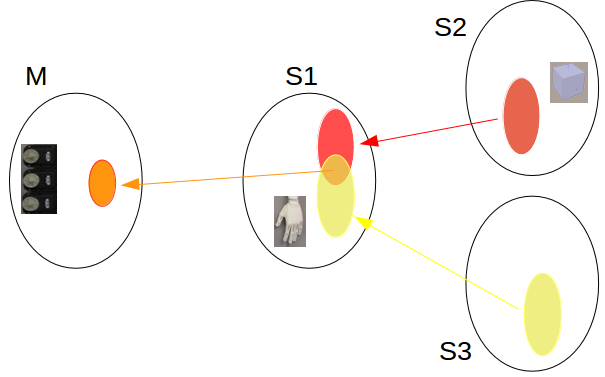
\includegraphics[width=12cm]{./include/tddriveext.png}
				\caption{Top-Down Drive to guide exploration of lower level models}
				\label{tddrive}
			\end{figure}


		%

			
		\subsubsection{Exploration of sensorimotor models of increasing complexity}
		\label{sec:increasing}
		
			\paragraph{}
			In the previous learning algorithms developed, 
			the hierarchy of models to learn is given to the agent as if it already knew the combinations of actions
			to explore in order to learn the successive tasks.
			We describe here an algorithm (Algorithm~\ref{algomult}) that autonomously generates different hierarchies of sensorimotor models and decides which of them to explore.
			To explore a hierarchy, it then uses the previously described algorithms that explore in a fixed hierarchy (e.g. Top-Down Drive, Sec. \ref{sec:interacting}).
			
			\paragraph{}
			Let $O = \{O_1, ...~ O_p\}$ be a set of operators allowed to combine the actions to reuse, for instance the sequence operator, that
			takes 2 actions and return the action that executes those 2 actions in sequence.
			Also, the parallel operator
			takes 2 actions and return the action that executes those 2 actions in parallel, when possible, and if the 2 actions take different values on 
			some motor, one of them is randomly chosen.
			
			\paragraph{}
			Given a set of motor spaces and sensori spaces (for instance vocal and arm motor spaces, visual and audio sensori spaces), the algorithm
			explores first the simplest sensorimotor models (e.g. $M_1S_1$, $M_1S_2$, $M_2S_1$, $M_2S_2$), and when making too small progress on those models
			complexifies the hierarchy of models.
			It then combine known models with the allowed operators to form a new more complex one (e.g. a sequence of an action in $S_1$ with the $M_1S_1$ 
			model and an action in $M2$, with $S_1$ as sensorimotor model).
			The algorithm increases the complexity of the hierarchies step by step, the complexity being the number of sensorimotor models 
			reused plus the number of sensori spaces used.
			
			\paragraph{}
			To decide which hierarchy to explore at each learning time step, a Multi-Armed Bandit algorithm monitors interest to explore (e.g. the competence progress) on each of them.
			The interest of a hierarchy is computed as the competence progress over the last experiments 
			on the models of that hierarchy (with a sliding window).
			
			\paragraph{}
			Each model can be used by several hierarchies that do not duplicate it but share it. Exploring a given hierarchy can thus benefits the other hierarchies.			
			This algorithm has not yet been implemented.
			
			
			\begin{algorithm}[H]
				\caption{Exploration of Sensorimotor Models of Increasing Complexity}
				\label{algomult}
				\begin{algorithmic}[1]
					\Require Motor spaces $M = \{M_1, ...~ M_m\}$
					\Require Sensor spaces $S = \{S_1, ...~ S_n\}$
					\Require Operators $O = \{O_1, ...~ O_p\}$
					\State \texttt{models\_MAB} $\gets$ MAB(list of models $(M_iS_j)$ with $i \leq m$ and $j \leq n$)~~~
					\Comment{Initialize a Multi-Armed Bandit with models of complexity $0$}
					\Loop
						\If{all models in \texttt{current\_models} are not interesting}
							
							\State \texttt{actions} $\gets M~\cup $ \texttt{models\_MAB}
							\State \texttt{combined\_actions} $\gets$ O(\texttt{actions} $\times$ \texttt{actions})
							\State \texttt{possible\_models} $\gets$ (\texttt{actions}$ ~\cup~ $\texttt{combined\_actions})$ \times P(S)$
							\State $c \gets$ max\_complexity(\texttt{current\_models})
							\If{some model of \texttt{models\_MAB}, has complexity $c$}
								\State \texttt{new\_model} $\gets$ a model of complexity $c$ from \texttt{possible\_models}
							\Else
								\State \texttt{new\_model} $\gets$ a model of complexity $c+1$ from \texttt{possible\_models}
							\EndIf
							\State add \texttt{new\_model} to \texttt{models\_MAB}
						\Else
							\State \texttt{model} $\gets$ Choose(\texttt{models\_MAB})
							\State Train(\texttt{model})
							\State Update \texttt{models\_MAB} with Interest(\texttt{model})
						\EndIf
					\EndLoop
				\end{algorithmic}
			\end{algorithm}

		%
		
		\subsubsection{Formulation as a Directed Acyclic Graph}
		\label{sec:dag}
		
			\paragraph{}
			The hierarchies of models can be formalized more efficiently, with a directed acyclic graph (DAG) that links motor and sensori domains and
			intermediate and top-level models (the models that are not reused by higher level models).
			Each model could then receive top-down drive from all the models from different hierarchies that reuse it, which would be more efficient that exploring independently the 
			hierarchies with the Top-Down Drive algorithm. See Fig. \ref{exemple} for an exemple of such hierarchies.
			In order to choose which model to explore, a tradeoff can be done for each model between autonomous interest and top-down drive and social guidance interests.
			The model to explore would then be the one with max tradeoff interest.
			
			

			\begin{figure}[H] 
				\centering 
				\begin{tikzpicture}[node distance=2.5cm,>=stealth',bend angle=45,auto]

					\tikzstyle{dom}   = [ellipse, thick, draw=black!75, fill=blue!20,  minimum height=10mm, minimum width=20mm]
					\tikzstyle{prim dom}   = [dom,  minimum height=15mm, minimum width=30mm,  fill=green!20]
					\tikzstyle{model} = [rectangle, thick, draw=black!75, fill=black!20, minimum size=15mm]
					\tikzstyle{top model} = [model, fill=red!20]

					\begin{scope}
						\node [prim dom] (pd1) {$M_1$};
						\node [prim dom] (pd2) [xshift=5cm] {$M_2$};
						
						\node [model] (m1) [above of=pd1] {$mod_1$}
						edge [pre]                  (pd1);

						\node [dom] (d1) [above of=m1] {$S_1$}
						edge [pre]                (m1);
						
						\node [model] (m2) [above of=pd2] {$mod_2$}
						edge [pre]                  (pd2);
						
						\node [dom] (d2) [above of=m2] {$S_2$}
						edge [pre]                (m2);
						
						\node [model] (m3) [above of=d1, label={[label distance=0.05cm]280:$O_1$}] {$mod_3$}
						edge [pre]                  (d1)
						edge [pre, bend right=20]                  (d2);
						
						\node [dom] (d3) [above of=m3] {$S_3$}
						edge [pre]                (m3);
						
						\node [top model] (m4) [above of=d2, label={[label distance=0.05cm]265:$O_2$}] {$mod_4$}
						edge [pre, bend left=20]                  (d1)
						edge [pre]                  (d2);
						
						\node [dom] (d4) [above of=m4] {$S_4$}
						edge [pre]                (m4);
						
						\node [top model] (m5) [above of=d3, xshift=1cm, label={[label distance=0.05cm]270:$O_2$}] {$mod_5$}
						edge [pre]                  (d3)
						edge [pre, bend right=10]                  (d2);
						
						\node [dom] (d5) [above of=m5] {$S_5$}
						edge [pre]                (m5);
						
						
						
						
					\end{scope}

					\begin{pgfonlayer}{background}
						\filldraw [line width=4mm,join=round,black!10]
						(d5.north  -| pd2.east)  rectangle (pd1.south  -| pd1.west);
					\end{pgfonlayer}
				\end{tikzpicture}

				\caption{Exemple of 2 hierarchies sharing models.
				Ellipses represent domains. Green ellipses: motor domains. Blue ellipses: sensori domains. Squares represent models. Gray squares: intermediate models. Red squares: top-level domains.	First hierarchy is composed of intermediate models $mod_1$, $mod_2$, $mod_3$, and top-level model $mod_5$.  Second hierarchy is composed of intermediate models $mod_1$, $mod_2$, and top-level model $mod_4$.
				}
				\label{exemple}
			\end{figure}


		%


		\subsubsection{Integrating social interaction}
			\label{sec:social}
			\paragraph{}
			We describe here different ways to integrate social interaction to those hierarchical learning architectures.				
			The following one is inspired from the SGIM-ACTS learning architecture \cite{nguyen2012}. 
			In SGIM-ACTS, the learning progress from each strategy are estimated. 
			The agent can learn autonomously, or learn in interaction.	
			When learning by interaction, the agent also learns from who to imitate, if teachers of different skills are available. 			
			For each model, we could thus estimate the interest of asking for teacher input (sensori tasks) on that model. 
			When the agent explores a given model, it then first chooses by which strategy to explore it: self-generation of goals, or teacher input, 
			and from which teacher to get the input that will serve as socially guided goal to imitate.

			\paragraph{}
			Another possibility is to merge the input from social peers with the interest distribution of the models.
			When generating a goal to explore for a given model, the interest distribution of the model is merged with the top-down drive interest distributions from higher models
			plus social interest given as a another distribution.
			
			\paragraph{}
			Also, if the social input is not specified at the goal spaces level, but more abstract, it could be integrated at the level of the choice of model or choice of hierarchy. 
			When choosing which hierarchy (in Algo. \ref{algomult} in the Multi-Armed-Bandit) or which model (in Algo. of Section \ref{sec:dag}) to explore, the agent could merge the interest with a social
			value or reinforcement for those hierarchies or models. 
			The implementation and evaluation of those different algorithms remains to be done.


		%

	%

	
	\subsection{Measures}

	
		\subsubsection{Exploration}
				
			\paragraph{}
			Exploration is a measure of how well the agent has found diverse outcomes in its task space. 
			It makes no assumptions about the interest of exploring given regions of the task space from the viewpoint of the engineer, 
			neither if we want the robot to learn specific tasks or if we know that certain tasks will be more useful later for the robot.
			To compute the quantity of exploration we consider the task space as a grid with small cells and count the number of cells that have been reached.
		
		%
		
		\subsubsection{Competence}
			\label{sec:competence}
			\paragraph{}
			Given a task region where we want to evaluate the competence of the agent, we draw random goals in that region and measure the distance of
			the point reached from that goal.
		
		%
		
		\subsubsection{Competent exploration}
		
			\paragraph{}
			As the agent self-generates goals in the task space, it might not yet have explored that evaluated part of the environment, 
			or in another run, have explored
			it very early, so it is hard to interpret this competence as a general progress.
			We thus define an intermediate measure that evaluates how well competent is the robot on the explored part of the task space.
			The competent exploration is thus the number of cells explored (as in the exploration measure) but that the robot can reach again,
			with some margin, when asked for it.
		
		%		
	 
		\begin{figure}[H] 
			\centering 
			\subfloat[]{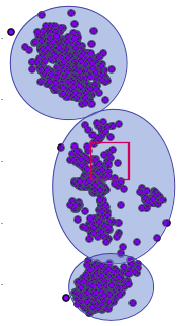
\includegraphics[height=7cm]{./include/measure_explo.png}}
			\hfil
			\subfloat[]{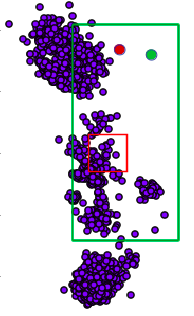
\includegraphics[height=7cm]{./include/measure_comp.png}}
			\hfil
			\subfloat[]{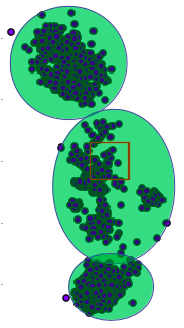
\includegraphics[height=7cm]{./include/measure_explocomp.png}}
			\caption{Measures of exploration. Blue points are 2D sensori points reached during exploration.
			(a) Exploration measures approximately the reached area (approx. the blue areas). 
			(b) Competence measures the ability to reach random goals in a task area (green rectangle) e.g. the green point is a goal, the red point is the reached position, leading to a high error for that goal. 
			(c) Competent exploration measures the ability to reach goals in the explored area (approx. green areas).}
		\end{figure}  	
	%

	
	\subsection{Environments}

		\subsubsection{V-rep simulated physical arm}
			
			\paragraph{}
			The experimental setup is composed of a robotic arm with $4$ degrees of freedom from the Poppy robot \cite{poppy} simulated with the V-REP simulator 
			based on the Bullet physics engine. 
			We use Dynamical Movement Primitive \cite{ijspeert_dynamical_2013} to control the arm's movement as this framework permits the production of a diversity of arm's trajectories with few parameters.
			Each arm's degree of freedom (DOF) is controlled by a DMP with a starting and a goal position equal to the rest position of the motor.
			Each DMP is parameterized by one weight on each of $5$ basis functions whose centers are distributed homogeneously throughout the movement of duration $4s$.
			The weights are bounded in the interval [-400,400] which allow each motor to cover its standard angle interval [-1,1] during the movement.
			Each DMP outputs a series of angle positions that represents a sampling of the trajectory of one motor during the movement.
			A block is placed near the robot's hand and can be moved in two dimensions in different complex ways, e.g. with the hand pushing on the top of the block or on a side, in one or two steps.
			We voluntarily kept the number of basis functions small for the agent to learn more easily the trajectory space but still being able to move the object in different complex ways. 

			
			\paragraph{}
			Let $M$ be the $20D$ space of the motor parameters and $S_h$ the $9D$ space representing the movement of the hand encoded by the projection of the $3D$ movement of the hand on DMPs with $3$ basis functions. 
			$S_o$ is the $2D$ space representing the position of the object at the end of the simulation.
			As we are interested in how an architecture has explored the different locations where the object can be pushed to, we define $S_o$ as the goal space where exploration will be evaluated.
			Thus, to evaluate the exploration of an architecture we compute the number of reached cells in a grid of $2cm$ width.
			And to measure the competent exploration, we draw one sample in each explored cell of the object space and use its sensorimotor model to infer a motor configuration that leads the object close to the given object goal position. We then run the movement in the simulator and check if the object has been moved less than $2cm$ away from the goal.
					
					
						

			\begin{figure}[H]
				\centering
				\subfloat[]{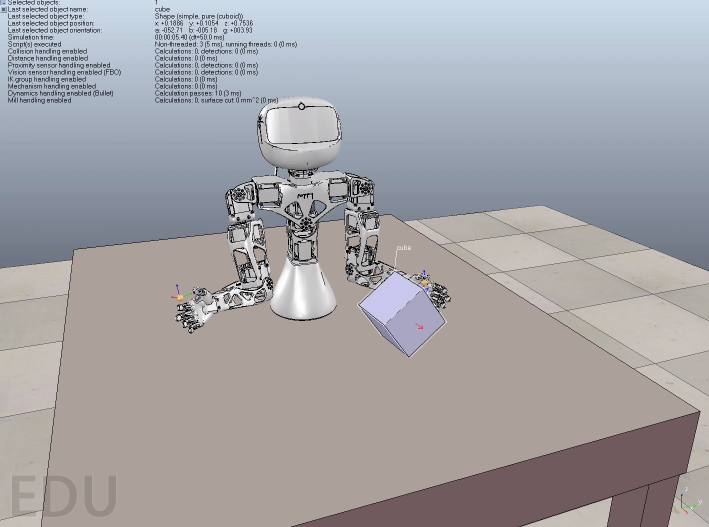
\includegraphics[width=12cm]{./include/torso.png}}\\
				\subfloat[]{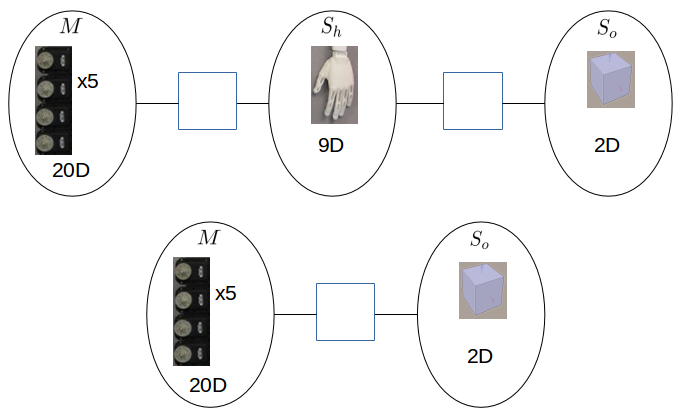
\includegraphics[width=12cm]{./include/scheme.png}}
				\caption{(a) Poppy Torso in the V-Rep simulator moving a block. (b) Top: Hierarchical architecture. Bottom: Control architecture.}
				\label{fig_sim}
			\end{figure}
			
		%
		
		\subsubsection{Simple geometric arm}
		
			\paragraph{}
			A simple geometric arm is defined as a $3$ DOF arm with a total length of $1$ unit, and the first part of length $4/7$ units, the second $2/7$
			and the last $1/7$. The sensori space has $2$ dimensions being the X and Y position of the end of the arm.
			
			\paragraph{}
			We also define new sensori objects in this environment as sliders that output a linear value between 0 and 1 if the end of the arm is close to the slider,
			and 0 if it is at a distance greater than $0.15$. For instance, in Fig. \ref{arms}, in (a) the 2 sliders output 0, and in (b), the first 
			slider outputs 0 and the second outputs $0.8$.
			
			\paragraph{}
			This environment will also be used in a sequence of 2 arm positions, with a new sensori value $s_3$ depending on $s_1$ and $s_2$ at the 2 timesteps:
			$$r1 = (s_1\_1 + s_2\_1)/2$$
			$$r2 = (s_1\_2 + s_2\_2)/2$$
			$$s3 = (r1+r2)/2 ~if ~r1 > 0 ~and~ r2 > 0 ~else ~0$$
			The new value $s_3$ then outputs a strictly positive value only if the arm has touched the 2 sliders in sequence.

			\begin{figure}[H]
				\centering
				\subfloat[]{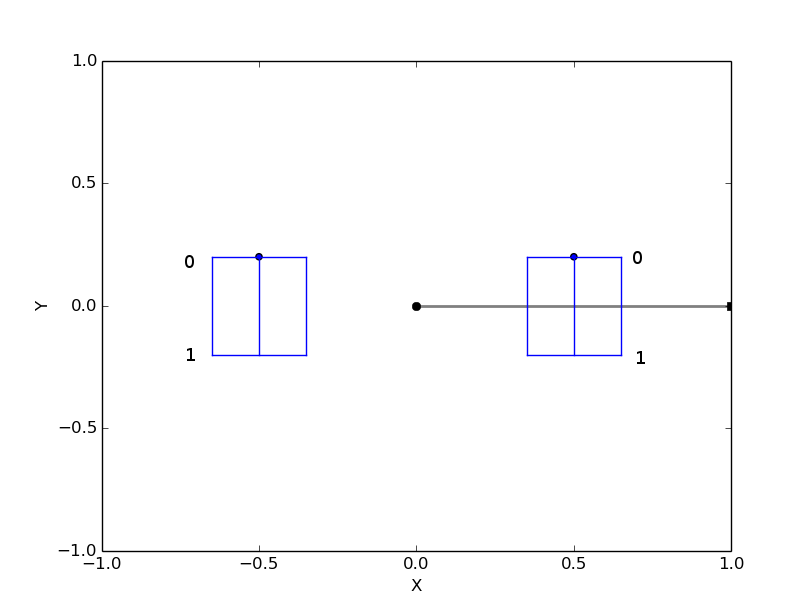
\includegraphics[height=2.62in]{./include/armseq1.png}}
				\subfloat[]{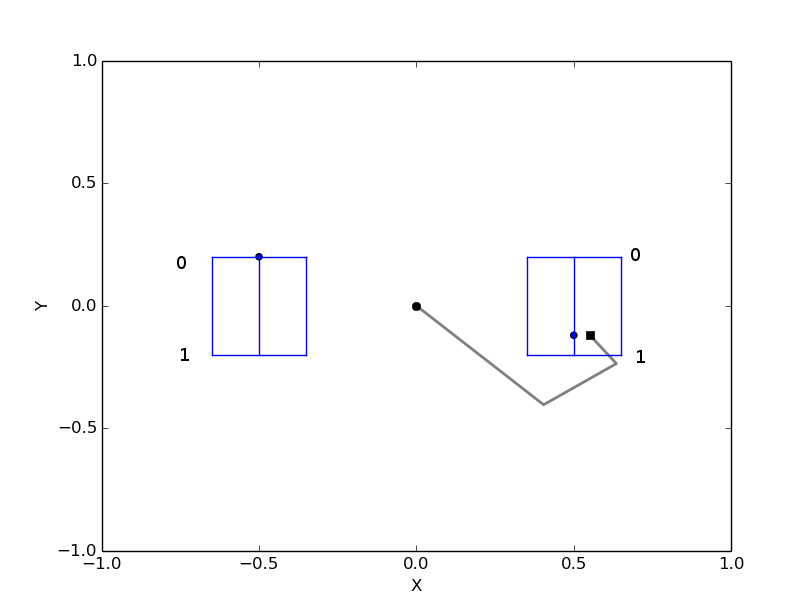
\includegraphics[height=2.62in]{./include/armseq2.png}}
				\caption{2 positions of the simple arm and corresponding values on the 2 sliders.}
				\label{arms}
			\end{figure}
			

		%

				
		\subsubsection{The DIVA synthesizer}

			\paragraph{}
			The DIVA synthesizer is a vocal synthesizer that outputs the formants of the sounds produced given the positions on $13$ motor values.
			As in \cite{moulin-frier_self-organization_2014}, we use only the first $7$ articulators, set the articulators 8 to 10 to 1 to ensure phonation,
			and articulators 11 to 13 to 0. We keep only the first and second formants as sensori output as they encode relatively well the vowels produces. 

			\paragraph{}
			We also add a slider as in the arm environment, as a third output value, between the sounds /o/ and /y/ with margin $0.3$ octave.
			
			\paragraph{}
			A combined environment is also defined where the arm with one slider $s_1$ and the vocal synthesizer with one slider $s_2$ are put together.
			A third output value is then computed as 
			$$s_3 = 4 \times (s_1 - 0.5) \times (s_2 - 0.5) ~if~ s_1 > 0.5 ~and~ s_2 > 0.5~ else~ 0$$
			
		%
			
			
		\subsubsection{Combination of arm and vocal movements}

			\begin{figure}[H]
				\centering
				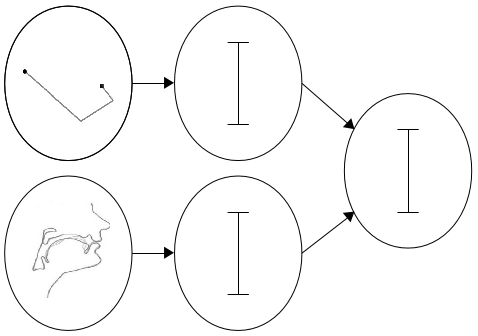
\includegraphics[width=10cm]{./include/multimodal.png}
				\caption{Multi-modal environment}
			\end{figure}
			
		%
			
	%
	
	
	\subsection{Experiments}

		\subsubsection{V-rep arm pushing a block}

			\paragraph{}
			In order to compare the first hierarchical architecture implemented, we test them on a simple hierarchical task where the robot arm simulated
			in V-rep has to push the block to different locations.
			We compare here the flat control architectures, the Simplest First, and the Top-Down guiding architectures, with goal babbling and SAGG-RIAC-like
			interest models. We measure the exploration and the competent exploration with a grid size of $0.02m$.

		%

		\subsubsection{Sequence of actions}

			\paragraph{}
			In order to compare the hierarchical architecture in a more complex hierarchical task with 2 lower models to learn before learning the high one, 
			we use simple arm environment with a sequence of 2 actions and the new output value $s_3$ depending on the value of the 2 sliders in the 2 actions.
			In hierarchical architectures, the first model learns a mapping between the first 3D $M$ action and the value on the first slider touched, the
			 second model learns a mapping between the second 3D $M$ action and the value on the second slider touched, and the high third model learns a 
			 mapping between the 2 sliders touched values and the $s_3$ new value.
			Flat architectures learn a mapping between the 2 3D actions and the 2 sliders and the new value, so a model of $M^2S_1S_2S_3$.
			We compare here the flat control architectures, the Simplest First, and the Top-Down guiding architectures, with goal babbling and SAGG-RIAC-like
			interest models. We measure the exploration on $S_3$ with a grid size of $0.001m$.
			

		%

				
		\subsubsection{Combination of arm and vocal movements}

			\paragraph{}
			In a similar mathematical problem but with a multi-modal combination of actions, we use the environment composed of a simple arm and a slider plus
			the DIVA synthesizer plus its slider.
			In hierarchical architectures, the first model learns a mapping between the first 3D $M$ action and the value on the slider, the
			 second model learns a mapping between the DIVA motor space and the value on the slider in formant space, and the high third model learns a 
			 mapping between those 2 sliders values and the $s_3$ new value.
			Flat architectures learn a mapping between the multi-modal 10D action and the 2 sliders and the new value, so a model of $M_1M_2S_1S_2S_3$.
			We compare here the flat control architectures, the Simplest First, and the Top-Down guiding architectures, with goal babbling and SAGG-RIAC-like
			interest models. We measure the exploration on $S_3$ with a grid size of $0.001m$.

		
		%
		
	%
	
		
\section{Results}

	\subsection{V-rep arm pushing a block}
	\label{result:tdd}
		\paragraph{}
		Preliminary results show comparable amounts of exploration for hierarchical and flat architectures 
		with the same SAGG-RIAC interest models (Fig. \ref{explo_vrep}).
		MS1 means that one single model learns the mapping between M and $S_h$. MS2 means that one single model learns the mapping between M and $S_o$ (flat control architecture).
		S1S2 means that one single model learns the mapping between $S_h$ and $S_o$. SEQ means that a model learns $MS_h$ in the first half and an other learns $S_hS_o$ 
		in the second half of the iterations (Simplest first strategy). TOP-DOWN-CMA means that the CMA evolution strategy is used in the model $MS_h$ to try to reach a hand movement 
		$s_h$ chosen by the model $S_hS_o$. TOP-DOWN-RANDOM means that around the $s_h$ chosen by $S_hS_o$, the first model makes 5 random explorations (taken into account in the 10,000 iterations).

		%\begin{figure}[H]
			%\centering
			%\subfloat[]{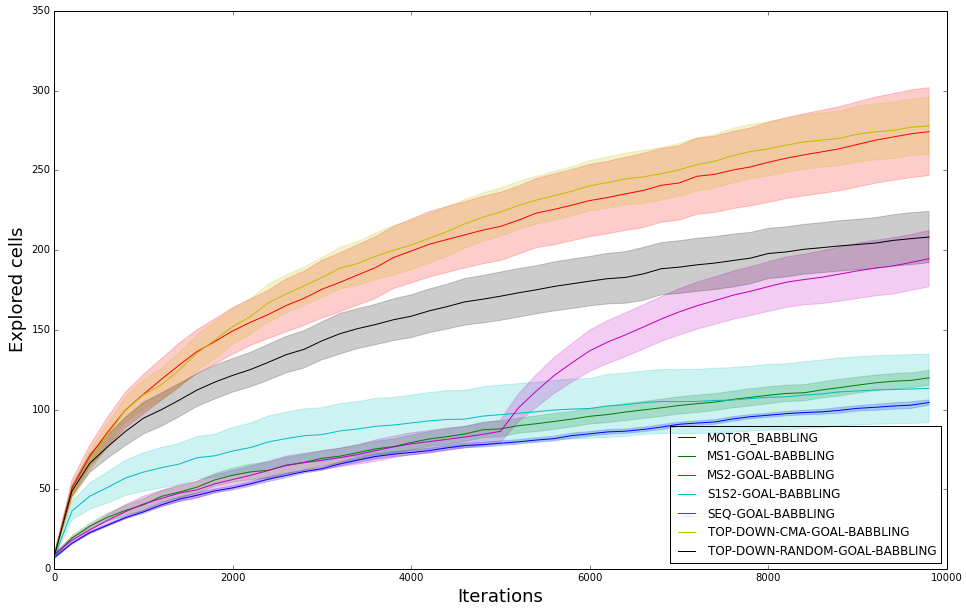
\includegraphics[height=4in]{./include/explo-2015-04-11_12-08-52_cube.png}}
			%\hfil
			%\subfloat[]{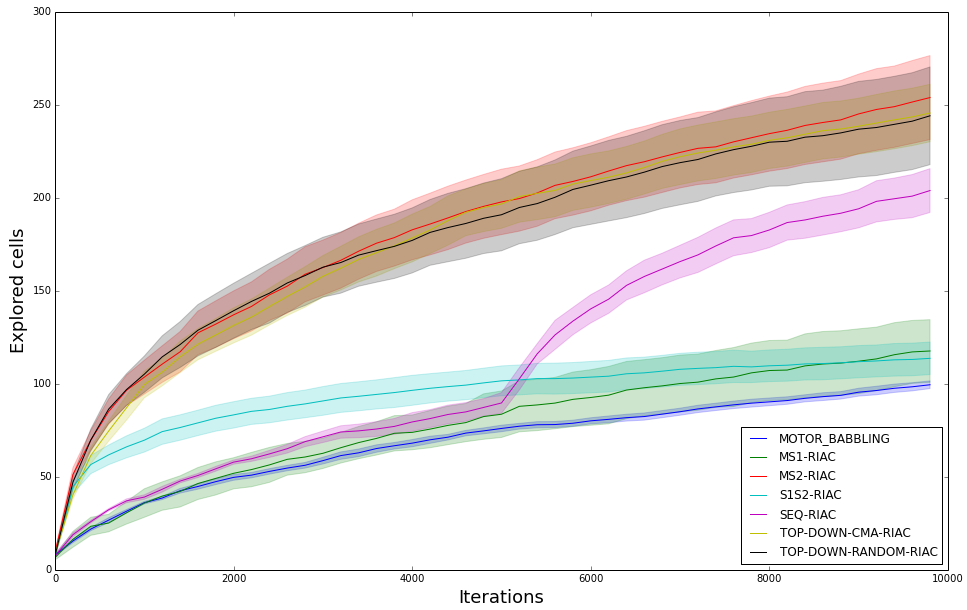
\includegraphics[height=4in]{./include/explo-2015-04-18_02-19-01-explaupoppydiva-riac-cube.png}}
			%\caption{Exploration in the object's space $S_o$. (a) SAGG-RANDOM exploration mechanism within models. (b) SAGG-RIAC.
					 %MS1: one single model learns the mapping between M and $S_h$. MS2: one single model learns the mapping between M and $S_o$.
					 %S1S2: one single model learns the mapping between $S_h$ and $S_o$. SEQ: a model learns $MS_h$ in the first half and an other learns $S_hS_o$ 
					 %in the second half of the iterations (Simplest first strategy). TOP-DOWN-CMA: the CMA evolution strategy is used in the model $MS_h$ to try to reach a hand movement 
					 %$s_h$ chosen by the model $S_hS_o$. TOP-DOWN-RANDOM: random exploration for $MS_h$ around the $s_h$ chosen by $S_hS_o$.}
			%\label{explo_vrep}
		%\end{figure}

		\begin{figure}[h]
			\centering
			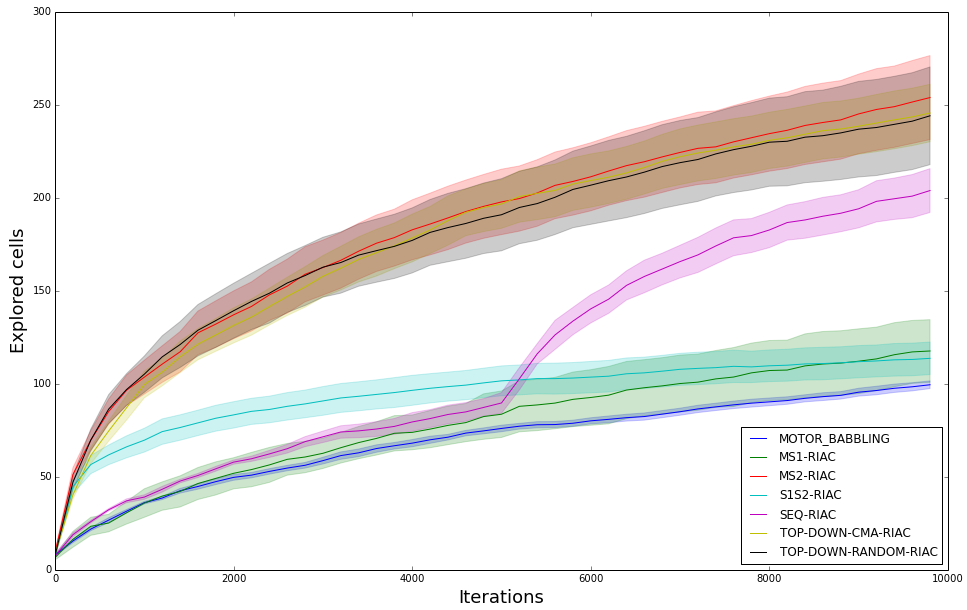
\includegraphics[height=4in]{./include/explo-2015-04-18_02-19-01-explaupoppydiva-riac-cube.png}
			\caption{Exploration in the object's space $S_o$ using the SAGG-RIAC interest model.
			Mann-Whitney U tests at the end of the experiments show that the exploration measures in the MS2, SEQ and TOP-DOWN conditions
			are significatively greater ($p<0.05$) than in the MOTOR-BABBLING, MS1 and S1S2 conditions.			
		}
			\label{explo_vrep}
		\end{figure}


		\paragraph{}
		As a very high variability results of the collision between the hand and the object, only a few explored cells, were in fact competent, in other words
		when we ask the robot to go to those cells,it succeeds in only a few.
		We measured the exploration together with the competent exploration in another run with a grid of size $0.1$ (Fig. \ref{explo_comp}).
		The competent measure is the number of cells where the robot succeeds in putting again the block at that place.
		
		\paragraph{}
		Mann-Whitney U tests at the end of the experiments show that the exploration measures in the CONTROL-GOAL-BABBLING and TOP-DOWN-GUIDANCE conditions
		are significatively greater ($p<0.5$) than in the SEQ condition, where it is significatively greater than in the CONTROL-MOTOR-BABBLING condition.
		On the other hand, tests on the competent exploration measure show that it is significatively greater in the TOP-DOWN-GUIDANCE condition than in 
		the SEQ condition where it is significatively greater than in the CONTROL conditions.

	
		\begin{figure}[H]
			\centering
			\subfloat[]{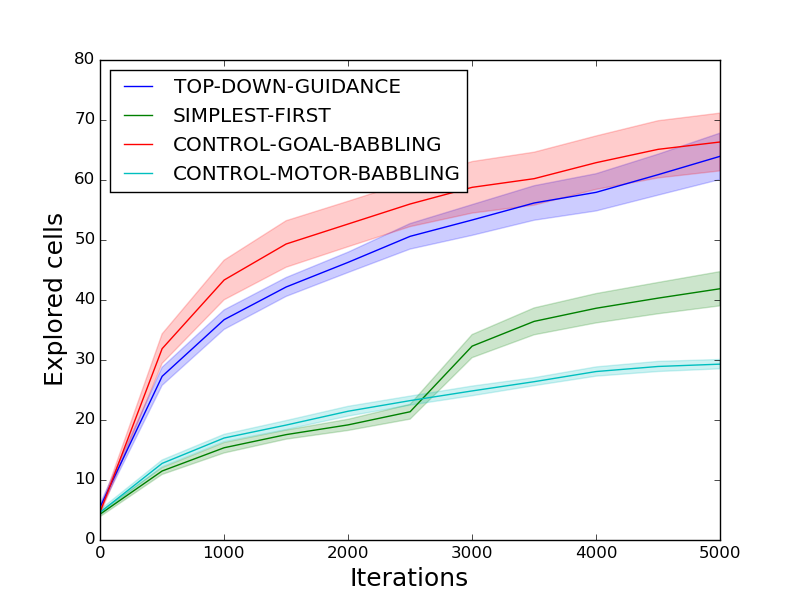
\includegraphics[width=3.5in]{./include/exploration_comparison.png}}
			\subfloat[]{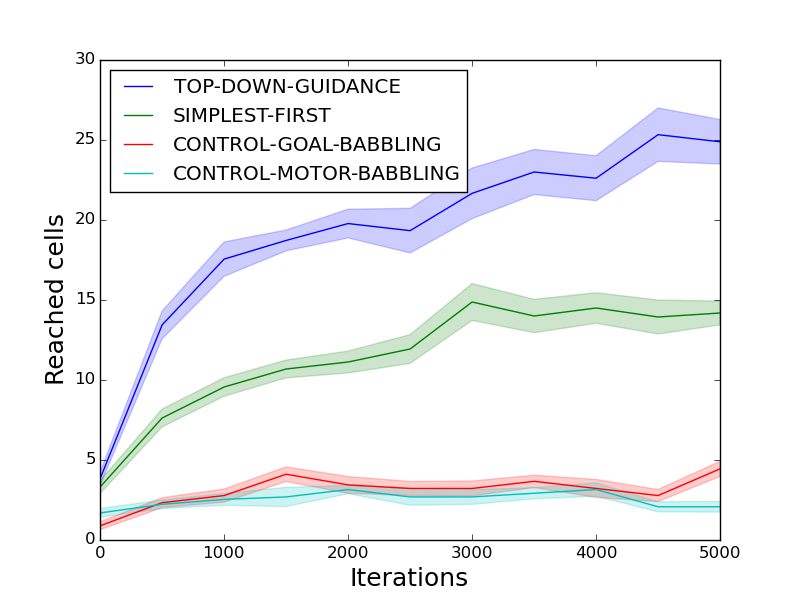
\includegraphics[width=3.5in]{./include/explocomp_comparison.png}}
			\caption{(a) Exploration. (b) Competent exploration. CONTROL-MOTOR-BABBLING: random motor parameters in $M$ are explored for all iterations. CONTROL-GOAL-BABBLING: one single model learns the mapping between $M$ and $S_o$. SEQ: a model learns $MS_h$ in the first half and an other learns $S_hS_o$ 
					 in the second half of the iterations (Simplest first strategy). TOP-DOWN-GUIDANCE: the CMA evolution strategy is used in the model $MS_h$ to try to reach a hand movement 
					 $s_h$ chosen by the model $S_hS_o$.}
			\label{explo_comp}
		\end{figure}

		
		\paragraph{}
		Results show comparable amounts of exploration for the top-down guidance and the control (goal babbling) conditions, whereas the competent exploration
		measure shows that the architectures learning an intermediate hand's movement representation allow the agent to put again the object on much more diverse
		locations. The intuition for this result is that when exploring around given motor parameters, the control architecture will modify some motor's angle trajectories and will produce more unstable interactions with the object than a hierarchical architecture that modify directly hand's Cartesian trajectory.
		A posssibilty to test this hypothesis is to choose an explored object's position $s_o$ in the condition TOP-DOWN-GUIDANCE, then infer a hand movement
		$s_h$ and then a motor set of parameters $m$ that should lead close to $s_o$. If the hypothesis is true, then given a variation $m'$ of $m$, and 
		an infered $m''$ of a variation $s_h'$ of $s_h$, the variance of the reached object position when repeating $m'$ should be higher than when 
		repeating $m''$.
		
		\paragraph{}
		Fig. \ref{diversity} shows the diversity of explored block position for the same experiment but several independant trials.
		This illustrates why measuring the competence (Section \ref{sec:competence}) does not make sense on a fixed subregion of the goal space as different runs
		do not explore the same parts of the space.
		
		\begin{figure}[H]
			\centering
			\subfloat[]{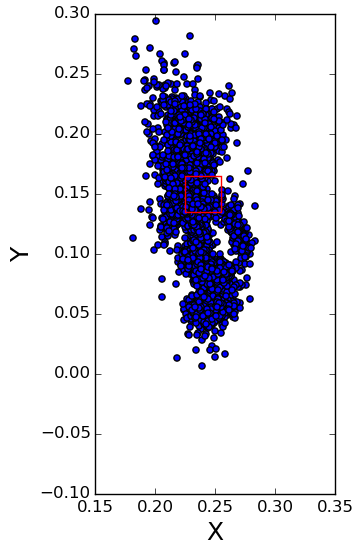
\includegraphics[height=2.4in]{./include/log1-scatter2D.png}}
			\subfloat[]{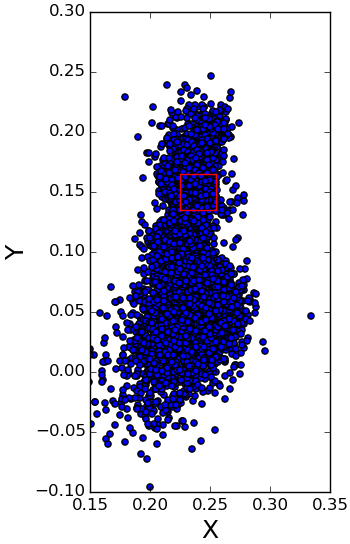
\includegraphics[height=2.4in]{./include/log2-scatter2D.png}}
			\subfloat[]{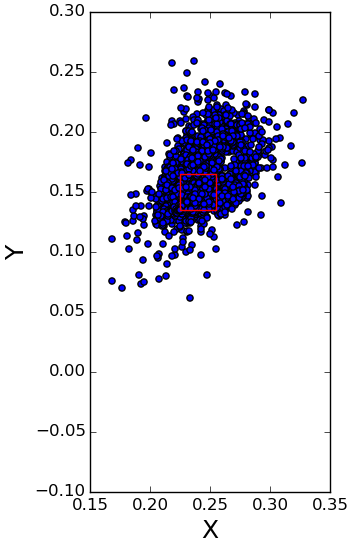
\includegraphics[height=2.4in]{./include/log3-scatter2D.png}}
			\subfloat[]{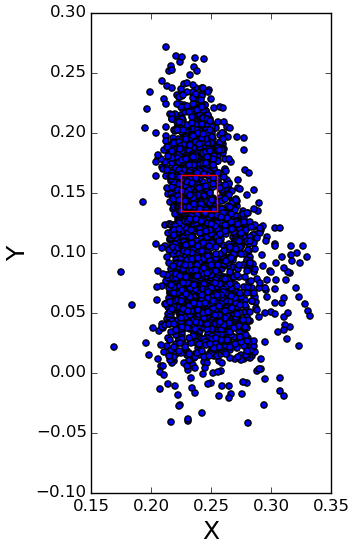
\includegraphics[height=2.4in]{./include/log4-scatter2D.png}}
			\caption{Variability in exploration in 2D space for several trials of condition TOP-DOWN-CMA-tree (SAGG-RIAC). Red square: initial position of the block.}
			\label{diversity}
		\end{figure}
		

	%
	


	\subsection{Sequence of actions}

		\paragraph{}
		Fig. \ref{explo_armseq} shows the results of the second experiment, with a sequence of 2 arm movements.
		Results show that the hierarchical Simplest First architecture explores better than the hierarchical Top-Down approach, which explores better
		than the flat architectures, either with goal babbling or SAGG-RIAC interest models.
		The motor babbling Simplest First hierarchical architecture explores also better than flat architectures.

	%


	\subsection{Combination of arm and vocal movements}

		\paragraph{}
		Fig. \ref{explo_armdiva} shows the exploration in the multi-modal arm plus vocal synthesizer environment.
		Results show that the hierarchical Simplest First architecture explores better than the flat architectures, 
		either with goal babbling or SAGG-RIAC interest models.
		The motor babbling Simplest First hierarchical architecture explores less than flat architectures.

		\begin{figure}[H]
			\centering
			\subfloat[]{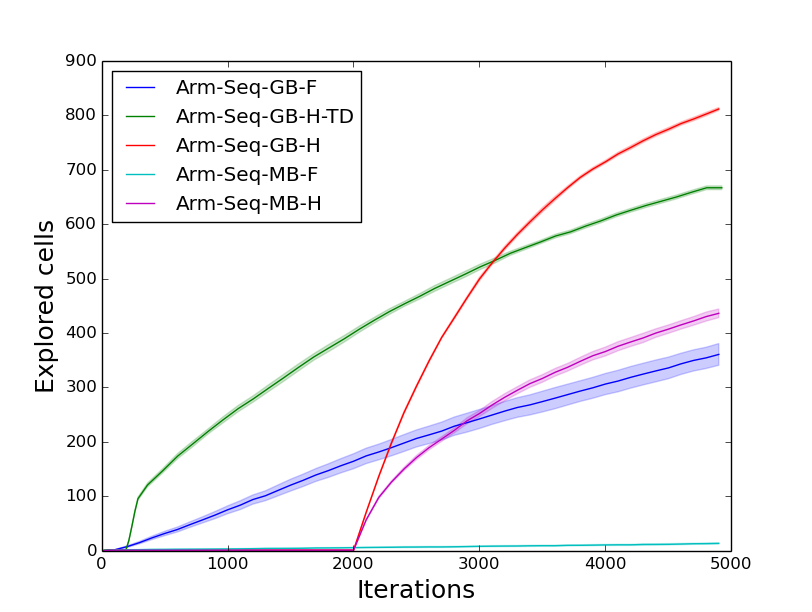
\includegraphics[height=3in]{./include/explo-2015-05-30_16-11-48-Test-Arm-Seq-GB.png}}\\
			\subfloat[]{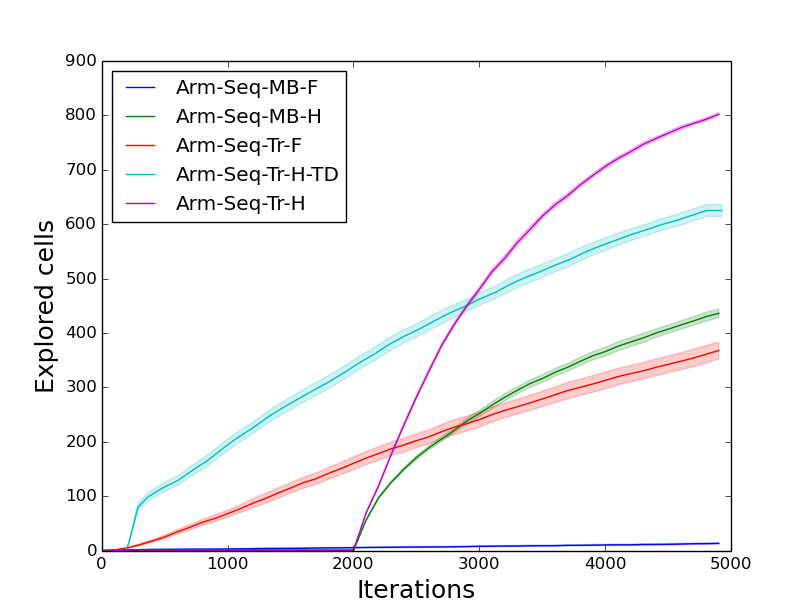
\includegraphics[height=3in]{./include/explo-2015-05-30_16-11-48-Test-Arm-Seq-Tr.png}}
			\caption{Exploration. (a) Goal Babbling versus Motor Babbling. (b) SAGG-RIAC versus Motor Babbling. GB: goal babbling is used to explore models. MB: motor babbling is used. Tr: SAGG-RIAC interest model. F: flat architecture with 1 model. 
					 H: hierarchical architecture with the Simplest First strategy with 3 models. GB-H-TD: GB is used to explore the high model, and TOP-DOWN-RANDOM to guide the 2 lower models. Tr-H-TD: SAGG-RIAC is used to explore the high model, and TOP-DOWN-RANDOM to guide the 2 lower models.
					 Mann-Whitney U tests at the end of the experiments show that the exploration measures in the GB-H and Tr-H conditions
			are significatively greater ($p<0.001$) than in the GB-H-TD condition where it is significatively greater ($p<0.01$) than in the Tr-H-TD condition, 
			where it is significatively greater ($p<0.001$) than in the MB-H condition, 
			where it is significatively greater ($p<0.01$) than in the Tr-F and GB-F conditions, 
			where it is significatively greater ($p<0.001$) than in the MB-F condition.}
			\label{explo_armseq}
		\end{figure}


		\begin{figure}[H]
			\centering
			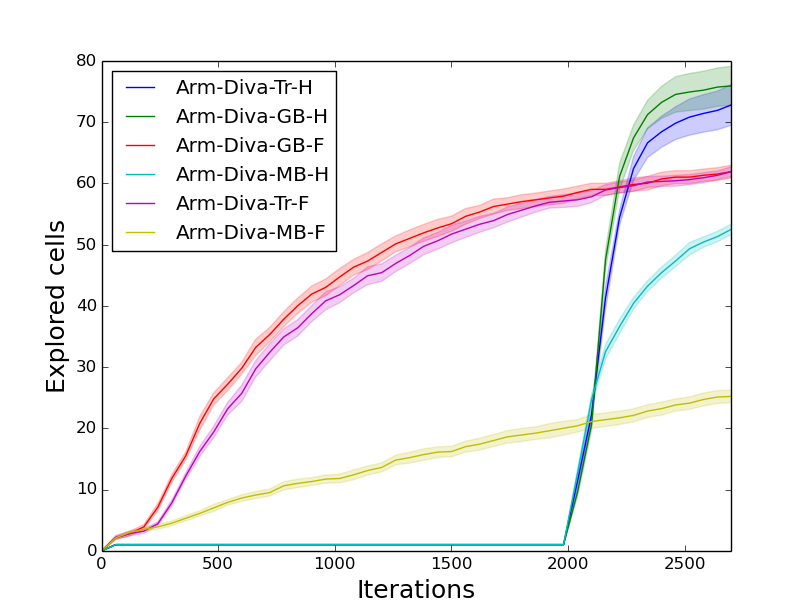
\includegraphics[height=4in]{./include/explo-2015-05-27_11-51-43-ARM-DIVA.png}
			\caption{Exploration in the multi-modal environment. GB: goal babbling is used to explore models. MB: motor babbling is used. Tr: SAGG-RIAC interest model. F: flat architecture with 1 model. 
			H: hierarchical architecture with the Simplest First strategy with 3 models.					 
			Mann-Whitney U tests at the end of the experiments show that the exploration measures in the Tr-H and GB-H conditions
			are significatively greater ($p<0.05$) than in the GB-F and Tr-F conditions,
			where it is significatively greater ($p<0.01$) than in the MB-H condition,
			where it is significatively greater ($p<0.001$) than in the MB-F condition.
					 }
			\label{explo_armdiva}
		\end{figure}

	%
	
	
%

\section{Discussion}

	\paragraph{}
	The hierarchical architectures composed of 2 models tested in the V-rep simulator show equivalent exploration results but better competent exploration than flat architectures.
	%This might first be due to the fact that in this case, the hierarchy does not help that much because it just allows the expression of the movement in 
	%an intermediate representation (the 9D projection of the hand movement) and is used only by one higher model. 
	%The picture should be different if several models were using the same intermediate learned representation.
	%Also, the benefits of an intermediate low dimensional hand movement space $S_h$ might not outweigh the downside of a too simple representation of the 
	%movement by the projection on sensory DMPs.
	
	\paragraph{}
	The results on the environment composed of a sequence of 2 simple arm commands and the multi-modal environment with an arm and a vocal synthesizer
	show that our exploration architectures get more useful as the hierarchy of sensorimotor models gets more complex.
	
	
	\paragraph{}
	The development of a parallel combination operator that allows to run different actions at the same time is not straightforward as a motor could receive two commands at the same time. 
	In that case,  a first idea is to randomly choose one of the commands.
	An interesting approach could make use of Probabilistic Movement Primitives \cite{paraschos2013probabilistic} that represent distributions of probabilities of movements on the different articulators.
	PMPs are shown to handle easily sequence and parallel combinations of movements as operations on distributions of probabilities, for instance the product of probability distributions for the parallel operator.
	%\paragraph{}%Stochasticité
	%In unstable environments, 
	
	\paragraph{}
	In the architectures developed (e.g. Section \ref{sec:increasing}), the sensori spaces represent environmental states that are received as input to the agent at the end of the executed actions.
	%Thus if several actions are combined in sequence, e.g. an action of model $mod_4$ in Fig. \ref{exemple} as a sequence $O_2(S_1, S_2)$ of an action of $mod_1$ and then an 
	%action of $mod_2$, the sensori state $s_1$ received by $mod_1$ could have been modified by the second action, leading to a wrong update of $mod_1$.
	In order to handle environments with hidden states, where sequences of actions have combinatorial effects, it should be beneficial to take the context of the action into 
	account, thus having contextual sensorimotor models relating an action $A$ in a sensori context $S$ to the next sensori state $S'$.
	The dimensionalities would then be much higher, which might require dimensionality reduction techniques.


	%
	
	
%


%\section*{Acknowledgment}

	%\paragraph{}
	%First of all I wish to express my sincere thanks to Pierre-Yves Oudeyer for his scientific guidance and his encouragements during this internship.
	%I am scientifically and personally pleased to be going to continue to work under his supervision for the more complex PhD task.
	%I would like to thank Jonathan Grizou and Fabien Benureau who gave me valuable advices and useful references.
	%I am also grateful to Pierre Rouanet who so kindly assisted me for all the technical questions.
	%Finally, I am grateful to William Schueller who gave me useful comments on previous versions of this manuscript and saved me crucial time.

%

%\newpage

	%
	
\section{Graph implementation}

	I'm trying to implement a first version of a graph representation of multiple hierarchies' learning.
	Before that, I have to be sure about the behavior of the SAGG-RIAC algorithm and its parameters 
	as it will be used as a sub-component in the multi-level graph representation.

	\subsection{SAGG-RIAC}
	\label{sec:saggriac}
		Here I want to study the important parameters of the SAGG-RIAC implementation 
		(from Explauto, with my implementation of RIAC in explauto.interest\_model.tree) and test them first on very simple environments.
		The goal is to get a sound progress output, that could be compared with other models' progresses.
		
		\paragraph{Parameters}
		\begin{itemize}
			\item sensorimotor model (KNN -default-, WNN, LWLR)
			\item exploration noise (gaussian noise amplitude -default $1/30$-)
			\item competence measure ($-distance$ or $exp(-distance)$, distance min -default=0.01-)
			\item progress measure (initial progress value, progress time-scale)
			\item leaf sampling mode (greedy, eps-greedy, softmax -default-), weighting by volume, no multi-scale sampling here
			\item constaints on tree: depth -default=6-, max number of points per region -default=100-
			\item split mode (middle -default-, median, best interest difference)
		
		\end{itemize}
		
		
		\paragraph{Questions}
		\begin{itemize}
	
			\item how does the progress measure evolve for very simple forward models ? (constant, piece-wise, linear, random)
			\item does progress change when split occurs ? (weighting by volume ?)
		
		\end{itemize}
	
		\paragraph{First Tests}
		\begin{itemize}
	
			\item \textbf{Constant forward model}. We have one motor dimension $m \in [0,1]$ and one sensory dimension always equal to $0~(\in [0,1])$.
				With default RIAC settings, the progress measure does not converge to 0, even if the distance min of the competence measure is not 0 (typically 0.01, which means that if the competence is better than 0.01 in the region, that region will become non-interesting).
				The reason seems to be that given a region not containing $0$ (e.g. $s \in [0.5-0.75]$), all the drawn goals will have a low competence 
				but varying between the competence of distances $0.5$ to $0.75$, with no amelioration with time.
				One idea to fix this problem is to set a maximum goal-to-reached distance (e.g. the size of the region) corresponding to a minimum competence, which will be the always obtained competence in our example, with no fluctuating progress.
				This idea works in this example, and is beneficial for the same reasons in the case of a \textbf{Random forward model}.
				However, in the case of a non-stationary forward model, a new kinematics too far from the learned one might not be computed as interesting (it might be at the beginning due to the time window).
				EDIT: That does not prevent adaptation to new forward models (See Fig. \ref{kmeans}).
				
			\item \textbf{Linear forward model}. We have one motor dimension $m \in [0,1]$ and one sensory dimension  $s = m$.
				The progress fluctuates between $0.1$ and $1$ for some hundreds iterations (learning phase) and then fluctuates at very low values ($10^{-2~to~-5}$)
				(stochastic changes).
				Setting a minimal distance in the competence measure (e.g. $0.01$) makes the progress go to stricly $0$ instead.
			
			\item Does progress change when split occurs ? 
				In order to have progress outputs comparable as possible between learning modules, 
				we should have a progress value that depends only on the new incoming data and not on a change in data representation.
				In the SAGG-RIAC algorithm, a split is decided when a region has too much points ($>100$ here).
				The progress of the 2 sub-regions is then recomputed with the competences of the 2 sub-sets of the points, separately.
				Assuming that the 2 sub-regions and the parent one have similar progresses, we have now 2 leaves with the same progress.
				In the sampling process, when we choose the leaf from which to sample a point with a softmax function applied to the interests, then 
				the 2 leaves will weigh 2 times more than the parent one, while representing the same region. 
				It might be interesting to explore more in splitted regions that need resampling, but that leads to a focuse on such regions that will thus be resplitted and so on, with too deep trees. I thus included a possibility to weight the interest of regions by their volume, which allow
				a more stable sampling process.
				
				
		\end{itemize}
		
		
	%
	
	
	\subsection{Hierarchical exploration}
	
		
		I implemented the hierarchical exploration of models with a model-first sampling (instead of a hierarchy-first).
		That mean I consider all the models to learn, see their learning progress, and sample one model with high progress 
		(with a softmax of relatively low temperature -$0.5$-). 
		Then that model goal babbles, chooses a motor configuration to try (add random noise), which can be in the sensory space of a lower-model level, 
		and execute the motor command (if no lower-level dependency) or give that goal to lower-level models to be executed now (with no exploration iterations budget, but allowing motor noise in lower-level models).
		A motor command $m$ is finally executed, and a sensory input $s$ observed.
		Each model is then updated with the dimensions of $ms$ it is concerned with, which can be different from what it asked to lower-level models.
		I also implemented the possibility to add an exploration budget around the top-down guided point, but I don't use it here as results are not clear.
		
		\paragraph{Parameters}
		\begin{itemize}
			\item model sampling (greedy, softmax -default-)
			\item sampling models (-default-) or first sampling the hierarchy to train (root of the DAG) and then the model in the hierarchy.
			\item add top-down guided exploration budget
		\end{itemize}
		
		
		\paragraph{Questions}
		\begin{itemize}
			
			\item In a simple hierarchy, do we see expected exploration behaviors ? e.g. if a model is harder to learn, is it babbling more often ?
					If a model is reusing another one, does a learning schedule autonomously emerge with the higher-level model explored significantly after ?
			\item For non-stationary forward models, the sensorimotor model does not forget old points. Should we weight also by time ?
		
		\end{itemize}
		
		
		\paragraph{First Tests}~\\
		I use here identity function as forward models.
		There are 2 low-level models (mod1 and mod2) and one higher level that only rely upon mod1.
		Thus $s1=m1, s2=m2, s3=s1$.
		In a second condition, the forward model of mod3 is changed at 5000 iterations with $s3=s1^2$.
		
		
		\begin{figure}[H]
			\centering
			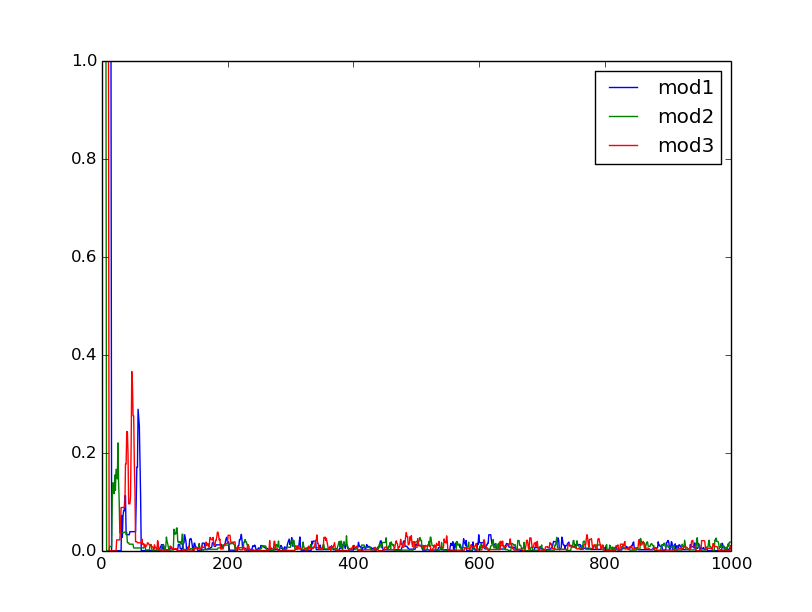
\includegraphics[width=8cm]{./include/Test_DAG_3mods_f=id-_1000.png}
			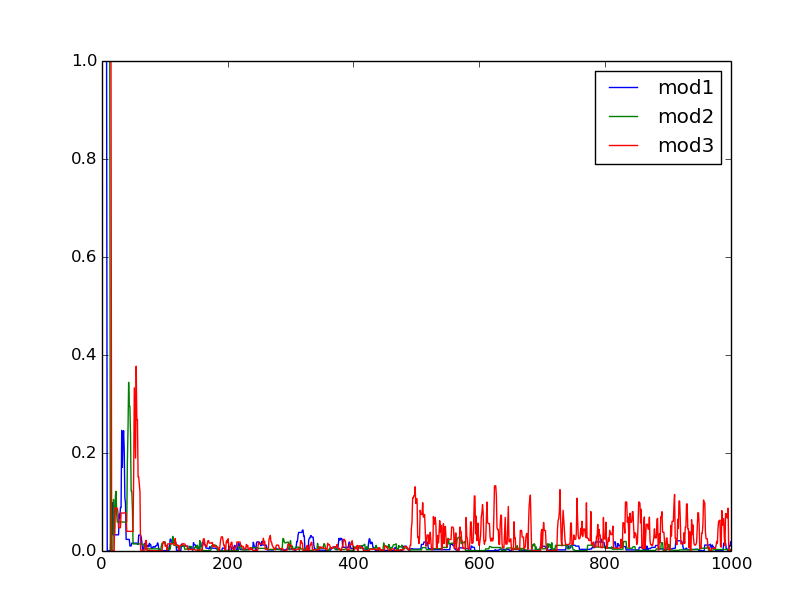
\includegraphics[width=8cm]{./include/Test_DAG_3mods_f=id_change_500-_1000.png}
			\caption{Exploration }
		\end{figure}
	
		\paragraph{Remarks}
		\begin{itemize}
			\item In the first condition, the 3 modules learn quickly their function, and then alternate. 
					In tests with more complex functions including random noise, the results are less clear (depend on max distance).
			\item In the second condition, at 5000, the 3rd module is seeing an increase in its progress but is not learning the change in its forward model.
					This is due to the problem described before, of non forgetting old sensorimotor points.
			\item In tests with a more complex hierarchy (7 models with some of them reusing several others), and a change in a given forward model, the results are similar.
			\item The progress or interest of a SAGG-RIAC tree is here computed as the progress on the last k (here $k=10$) babbling points on the overall tree, taking the points of all leaves into account (default).
					Another way to compute the progress is to get the maximum of the progress of each leaf. This does not change qualitatively the results.
		\end{itemize}
		
	%	
	
	\subsection{More on Non-Stationary Forward Models}
	\label{NSLWLR}
	
		\paragraph{}
		To cope with non-stationary forward models, with have to somehow forget old points and consider more the newest ones.
		The linear regression in LWLR is weighted by the distance of the points in the dataset. We can also weight them according to their timestamps (iterations at which the points were added).
		Given $x$, we want to compute $f(x)$, using data points $\{x_i, y_i\}$.
		First idea: we compute the weights of the Locally-Weighted Linear Regression with:
		
		$$ w_i = K_g(dist(x_i, x), \sigma^2) * ((iteration(i) - min\_iteration +1)/max\_iteration)^2$$
		where $K_g$ is a gaussian kernel with $\sigma = 0.05$.
		
		The results (Fig. \ref{NS1}) do not show a stabilization of the progress towards $0$ after the change in forward model at iteration $500$ for module $3$.
		
		\begin{figure}[H]
			\centering
			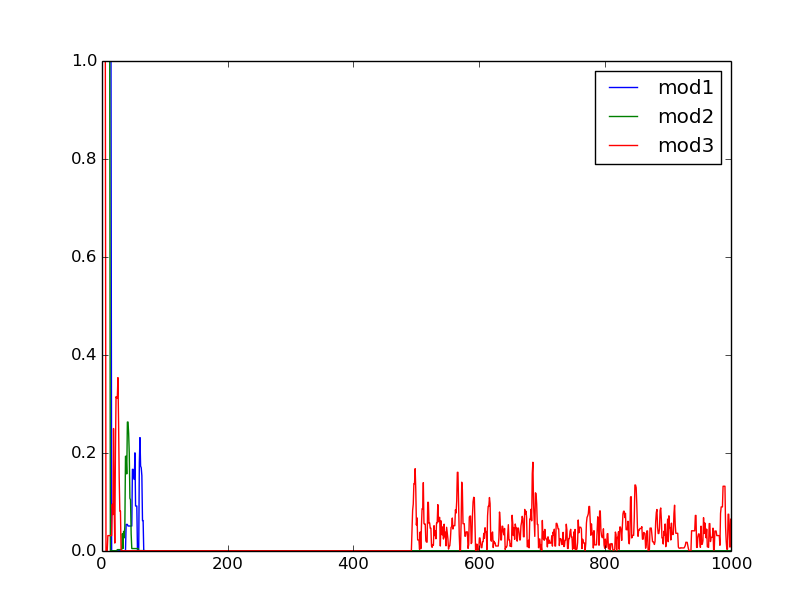
\includegraphics[width=8cm]{./include/NSLWLR-k=05.png}
			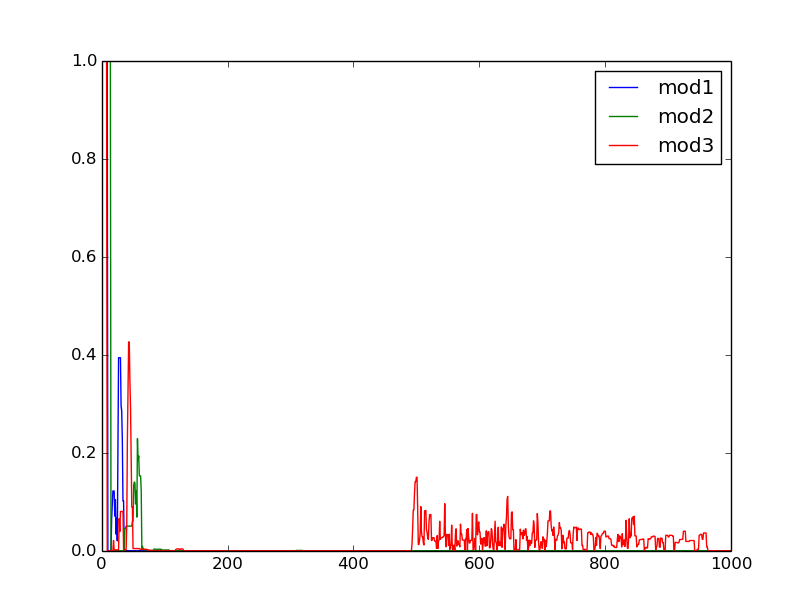
\includegraphics[width=8cm]{./include/NSLWLR-k=20.png}
			\caption{Progress of the 3 modules. The weights of the LWLR regression are weight with iterations' timestamps. Left: k=5 points used in regression, Right: k=20 points. Progress is measured as the max of the progress of each leaf.}
			\label{NS1}
		\end{figure}
		
		\paragraph{}
		Second idea: we use a gaussian kernel also for time weighting (see Fig. \ref{gt}, left).
		$$ w_i = K_g(dist(x_i, x), \sigma^2) * K_g(current\_iteration - iteration(i),~\sigma_t^2)$$
		with $\sigma_t = 100$ iterations.
		
		The result is shown in Fig. \ref{gt} left.
		That was neither a fast adaptation so I closer looked into the progress depending on the leaves. 
		I saw that the non-zero progress was due to the initial guess point of the inverse optimization (with algo L-BFGS-B) that was set as the $x$ corresponding to the nearest neighbor of the goal $y_g$ in the dataset.
		After the change in forward model, the guess point is often corresponding to the old forward model, and the optimization starting with that points is often failing, returning uncertain or 0 values giving a not real progress to the leaf.
		I changed the number of initial guess points (goal's nearest neighbors) to try with inverse optimization to $k=10$ (Fig. \ref{gt} right).
		Now, if points corresponding to the new forward model do exist near the goal, they are tested and optimization fail much seldom.
		However, the computation time gets too long.
		
		\begin{figure}[H]
			\centering
			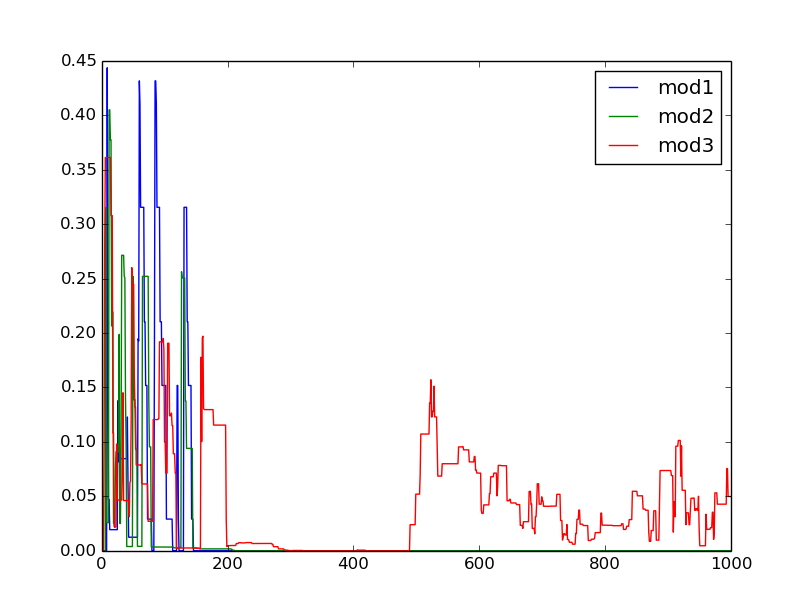
\includegraphics[width=8cm]{./include/NSLWLR-opt_k-initial=1.png}
			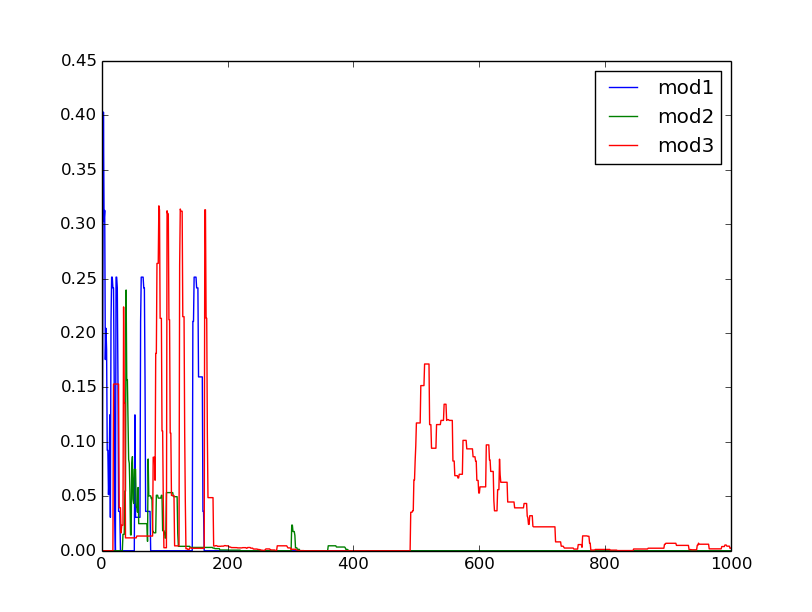
\includegraphics[width=8cm]{./include/NSLWLR-opt_k-initial=10.png}
			\caption{Progress of the 3 modules. The weights of the LWLR regression are weight with a gaussian time kernel. Left: 1 point is used as initial guess. Right: 10 points are used. Progress is measured as the progress on the last points of the global tree.}
			\label{gt}
		\end{figure}
	
		\paragraph{}
		An idea is to try only different points (ideally one old point and one new point) from the dataset as initial guess to the inverse optimization.
		I did that with a k-means clustering of the $50$ nearest neighbors of the goal in the dataset, to get 2 clusters. The inverse optimization is feeded with the 2 clusters' centroids as initial guess.
		The results (Fig. \ref{kmeans}) show the same adaptation as the $k=10$ guess points (Fig. \ref{gt} right) but is much faster.		
		
		
		\begin{figure}[H]
			\centering
			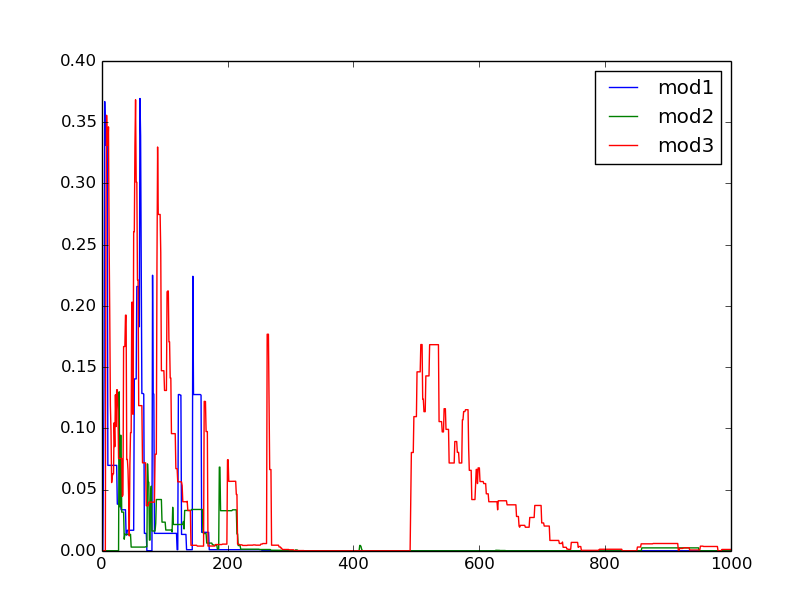
\includegraphics[width=8cm]{./include/NSLWLR-kmeans2-k=50_max_prog.png}
			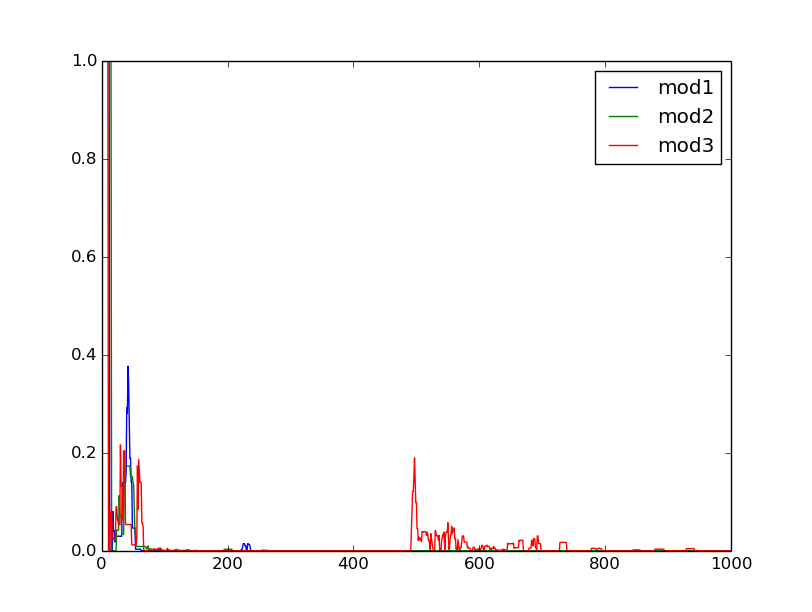
\includegraphics[width=8cm]{./include/NSLWLR-kmeans2-k=50_all_prog.png}
			\caption{K-means clustering of 50 initial guesses in 2 clusters to try inverse optimization. Left: Progress is measured as the progress on the last points of the global tree. Right: Progress is measured as the max of the progress of each leaf.}
			\label{kmeans}
		\end{figure}
		
		There is still some noise due to BFGS failed optimizations that sometimes sticks to the domain bounds, which gives competence noise in the SAGG-RIAC tree's lowest leaf (e.g. with bounds [0-0.125] -tree max depth is $3$ here).
		The adaptation is satisfying, given that the time kernel size is of $100$ iterations. In Fig. \ref{gt20}, the gaussian time kernel has size $20$ iterations, and different forward model's transitions are tested.
		The transition from a harder to a simpler forward model seems to need longer adaptation, but it might not be significant.
		
		\begin{figure}[H]
			\centering
			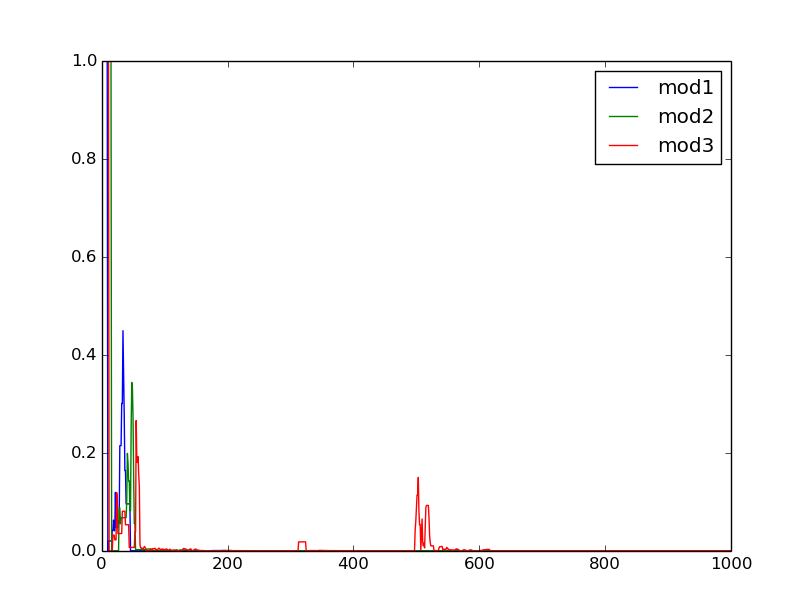
\includegraphics[width=8cm]{./include/NSLWLR_gt20_hard-easy.png}
			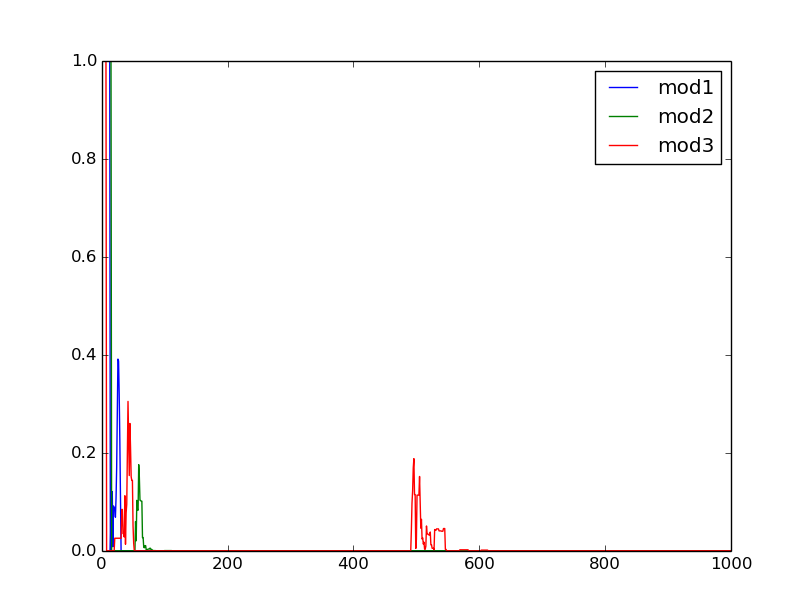
\includegraphics[width=8cm]{./include/NSLWLR_gt20_easy-hard.png}
			\caption{Progress on the 3 modules. LWLR weighted with a gaussian time kernel of size $20$ iterations. Left: forward model of module $3$ moves from $x\rightarrow x^2$ to $x\rightarrow x$.
			Right: forward model of module $3$ moves from $x\rightarrow x$ to $x\rightarrow x^2$.}
			\label{gt20}
		\end{figure}
		
		
		When one module see a change in its forward model, all the models that reuse it will not have their sensorimotor model modified, but will have their interest model perturbated.
		For instance, let's say module $1$ learns the mapping from $m_1$ to $s_1$ and becomes wrong, and module $2$ learns a mapping from $s_1$ to $s_2$ and reuses module $1$.
		Then when module $2$ is babbling, it wants to produce $s_2$ so infers a $s_1$ to try, and feeds it to module $1$ that fails at producing $s_1$ but produces instead $s'_1$ that leads to $s'_2$ far from $s_2$. 
		Thus both modules see a decrease in competence and thus an increase in interest.
		
		\paragraph{}
		As all models reusing the perturbated one gets a perturbated interest (interest that do not actually correspond to a change in the competence of the model's mapping), thus a lot of exploration iterations might be wasted
		on those models while they do not necessarily need training.
		With 4 models in a linear hierarchy where model $i+1$ reuses model $i$, Fig. \ref{f10} left shows the results after a change in the forward model of module $1$ at iteration $200$.
		Indeed, the $4$ modules have a non-zero interest and are sampled, from iterations $200$ to $300$, whereas only module $1$ needs sampling.
		An idea to avoid this waste of exploration is to weight the interest of each module (before a softmax choice) depending on the level of modules in the hierarchy.
		I used the following weights in Fig. \ref{f10} right: 
		
		$$ w_{mod_i} = p_i * f^{max\_level - level(i)}$$
		
		where $p_i$ is the progress of module $i$, $f$ a power factor, $level(i)$ is the level of module $i$ in the hierarchy: from $0$ for module $1$ to $3$ for module $4$.
		
		We can see in Fig. \ref{f10} right that even if modules $3$ and $4$ have sampled a few points between iterations $225$ and $400$, most of the babbling is done by module $1$ that corrects its own sensorimotor model.
		This idea to first train on more basic skills seems ecological and can be applied to more complex hierarchies, and can also be combined with other mechanisms to choose modules to train.
		
		
		\begin{figure}[H]
			\centering
			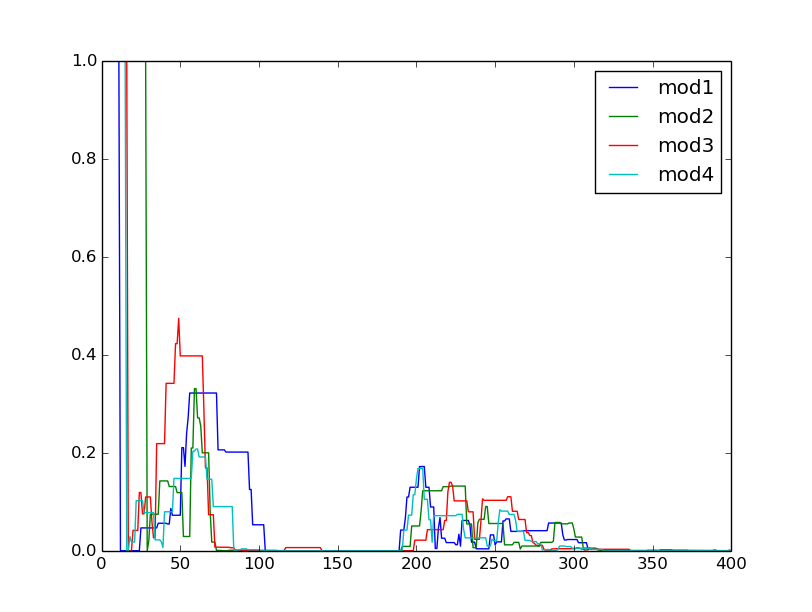
\includegraphics[width=8cm]{./include/NSLWLR-f=0.png}
			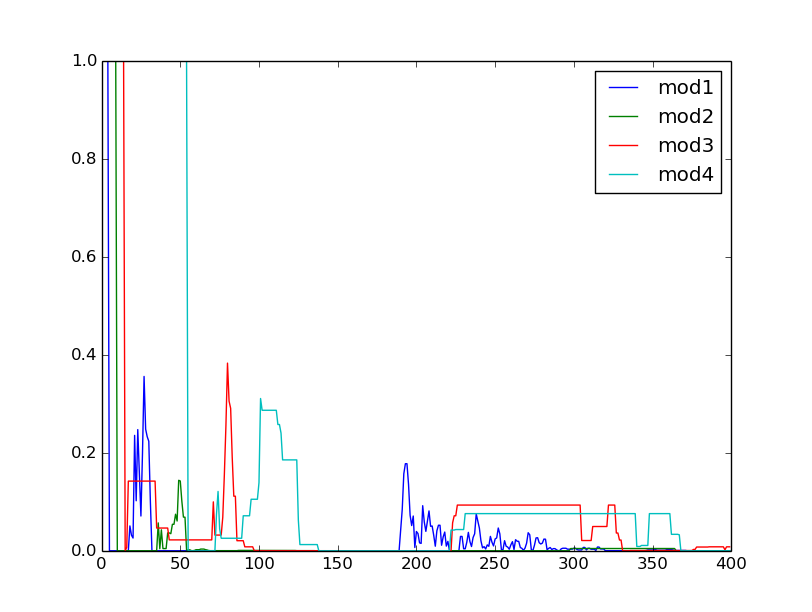
\includegraphics[width=8cm]{./include/NSLWLR-f=10.png}
			\caption{Progress on the 4 modules of a linear hierarchy. Left: $f=0$. Right: $f=10$.}
			\label{f10}
		\end{figure}
		
		
	\subsection{Creation of modules/tasks}
	
		
		\paragraph{}
		Here we allow the creation of modules when all the progresses of current modules are below a threshold (e.g. 1e-2).
		
		\paragraph{Module creation}
		An operator is randomly chosen among the concurrence and sequence operators.
		Then, 2 input connexions are chosen among the output of other modules plus primitive motor spaces.
		A sensory space is randomly chosen as a subset of all possible sensory spaces.
		In case of the concurrence operator, there are constraints on the input and output spaces: that the 2 input's set of controled variables must have a void intersection, 
		and that the motor spaces can't be in the sensory spaces.
		We could remove the constraints and let the agent understand that this module might be useless, but it could be a waste of iterations.
		
		\paragraph{}
		In the following experiments (see Fig. \ref{pc}), we use the previous linear hierarchy as initial models (from module 1 to module 4), and we use the constraints above for the concurrence operator.
		As we have only one motor space, the concurrence operator constraints can't be fulfilled, so the sequence operator only will be chosen.
		
		
		
		\begin{figure}[H]
			\centering
			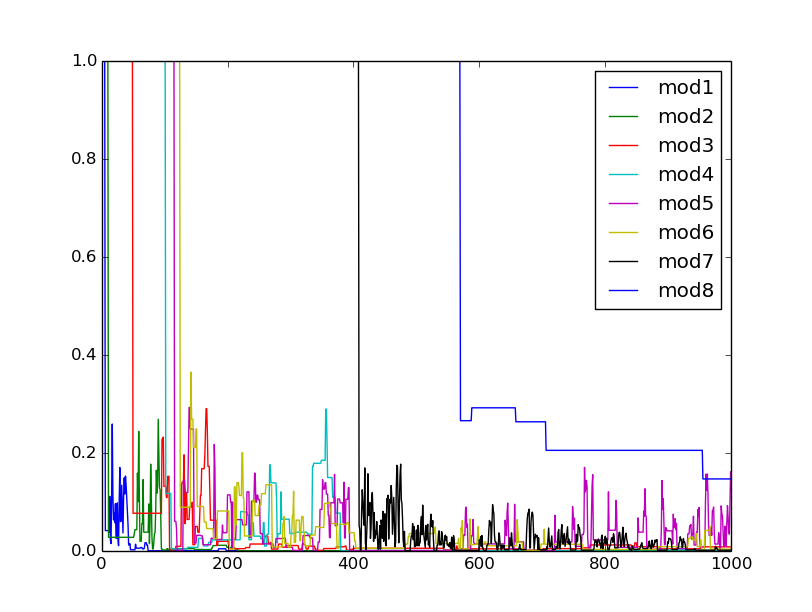
\includegraphics[width=8cm]{./include/autocreate_progresses.png}
			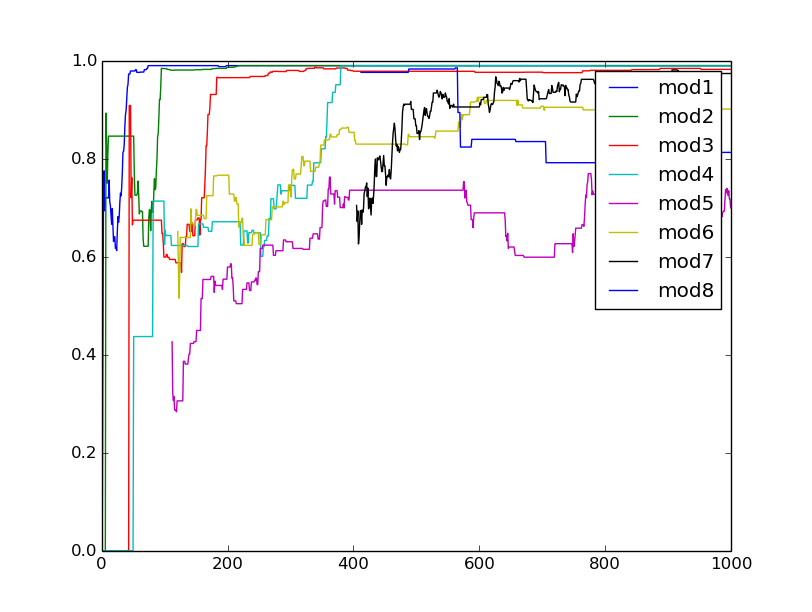
\includegraphics[width=8cm]{./include/autocreate_competences.png}
			\caption{Left: Progress of modules. Right: IM Competence of modules: competence to reach self-generated goals, which depends on the sensorimotor competences of involved modules.}
			\label{pc}
		\end{figure}
	
	
	
	%
	
		
	\subsection{More on Top-Down Drive}
	\label{tddkdtree}
	
		\paragraph{}
		The idea of Top-Down Drive is that higher modules in the hieararchy have relevant information about the utility of the exploration of the different regions of the common representation space.
		Different ideas might allow to take this information into account.
		In the experiments with the V-rep arm pushing a block (\ref{result:tdd}), I suggested 2 possibilities (See Section \ref{sec:interacting}).
		One is that each module asked to reach a goal, explores with a small budget of experiments around that goal before infering a motor command to reach that goal.
		A problem with that approach is that in a complex hierarchy, it would take to much time to infer a motor command for a goal containing a lot of nested sub-goals, 
		furthermore as each module could receive multiple goals.
		The second approach, not implemented was thus to feedback a top-down interest model in the common space to lower models that will have to balance 
		the self-computed interest map with Top-Down interest map (and even social interest map).
		The drawback now is that a lot of maps represented for instance with GMMs have to be handled, recomputed, multiplicated and sampled.
		
		\paragraph{Weighting by the density of Top-Down goals.}
		An other approach in-between would be to store, for each module, all the goals that have been asked from higher models in a specific KDTree 
		(different from the SM model that contains all points, and from IM model that contains the self-generated points).
		The information of interest to explore a point would be retrieved as the density of points in the kdtree around the given point.
		This could be computed with sklearn.neighbors.KDTree.kernel\_density that takes the bandwidth of a gaussian kernel as input.
		
		In order to balance self-computed interest with Top-Down interest, we could include the Top-Down information into the softmax choice of a leaf of the interest model's tree (in SAGG-RIAC) to explore.
		Up to now, the weights of the leaves are the competence progress on the points of each leaf.
		The idea is to also weight the interest of the leaves by the density of the Top-Down points around the center of each leaf.
		The bandwidth of the gaussian kernel could be proportional to the leaf's size as that is the relevant scale to smooth density information.
		
		In the case where we do not use SAGG-RIAC but SAGG-Random, instead of sampling random goals, we could directly sample the density map (implemented in sklearn) most of the time, and randomly sample sometime.
	
			
		\paragraph{Taking into account the information of the error between desired and actual motor command.}
		With the previous algorithm based on the density on Top-Down asked goals, there still exists information not handled but which might be useful.
		Indeed, when a module asks for a desired motor command $m_d$, if lower modules do not reach that goal but a $m_r$ potentially far from $m_d$, 
		then the distance $e_m = ||m_r - m_d||$ represents the error of lower models and might be useful to drive their exploration.
		The density idea already uses the information of the point $m_d$, but not the associated $e_m$ which could lead to a quantity of progress if derived.
		This learning progress is exactly the learning progress computed in a leaf of the interest model of lower modules, but there it is updated only when that sub-module has babbled, 
		not when a higher module has asked for a goal. If we were to update also the interest models when modules have not babbled, I guess that would mess up the competence derivative computation, leading to wrong estimates.
		So I don't know if we can use this supplementary information.
		
			
		\paragraph{Taking into account the progress in the leaf of the remote module that has been babbled.}
		In the density algorithm above, when a higher module has asked for a goal $s_g$, that point is added to the density map of Top-Down goals, 
		saying that this point is an interesting location to further explore around.
		But overall, some of those asked goals will lead to a progress in a leaf of the remote module that has babbled, and some of them will not.
		Thus it might be useful to use that information to add or remove interest in the given region of the map of Top-Down goals depending on the progress that has been remotely elicited.
		To this purpose, we could inspire from the framework of RL and particularly the $TD(\lambda)$ algorithm that makes use of eligibility traces that stores the influence of each state on the future reward.
		We could see the progress computed in the leaf that has babbled as a reward which will be added to the Top-Down interest of the leaves that have been used in the given command 
		(with accumulating or replacing eligibility traces).
		
		This idea is also inspired by the RiARiT algorithm that stores a table of competence levels required by each activity on each knowledge component.
		Each knowledge component thus knows the influence it has on each activity.
		In our setting, knowledge components are themselves activities, and that table would be estimated on-the-fly and at the leaf scale.
		
		The implementation would use the mean of (possibly time-decaying) rewards in each leaf as a weight to be balanced with self-computed leaves' interests before a leaf softmax choice.
		
		
		
		
	%
	
		
	\subsection{Implementation of multiple options to explore a given sensori space}
	\label{choices}
		
		\paragraph{}
		I have implemented the possibility to have different modules that learn a mapping towards the same sensori space.
		A higher module that uses that space as a motor space will choose which lower module to use to explore a point in that space with the goal to maximize the competence around that point.
		I have tested that idea using SAGG-Random modules instead of SAGG-RIAC ones.
		I compute the progresses (to choose the module that will babble) as the derivative of the competence of last goal babbled points.
		The competence around a point (to choose the module that will reach the goal with the maximum precision) is computed as the mean of the competences of the $k=20$ nearest neighbors.
		
		\paragraph{}
		The hierarchy used is the following: mod1 learns from $m1$ to $s1$, mod2 learns from $m2$ to $s1$, and mod3 learns from $s1$ to $s2$.
		Mod3 can thus reuse either mod1 or mod2. All spaces are 1-dimensional with range $[0-1]$. Here are the forward models:
		
		$$s1 = \frac{2*m1 + m2}{3}$$
		$$s2 = s1^2$$
		
		Thus, if mod3 reuses mod1, it will reach a wider range of outputs than with mod2. Fig. \ref{fchoices} shows the results of 2000 iterations with this setup.
		Mod3 quickly (100 iterations) gets to use mod1 (around 90\% of babbling iterations) instead of mod2.
		In the computation of competences, I also cut the competences to a minimal competence value (or maximal error distance of $0.1$) in order to avoid big random fluctuations of interest (absolute value of progress) 
		when a module wants to explore a far unreachable point, which entails a very high interest (see Sec. \ref{sec:saggriac}).
		
		\begin{figure}[H]
			\centering
			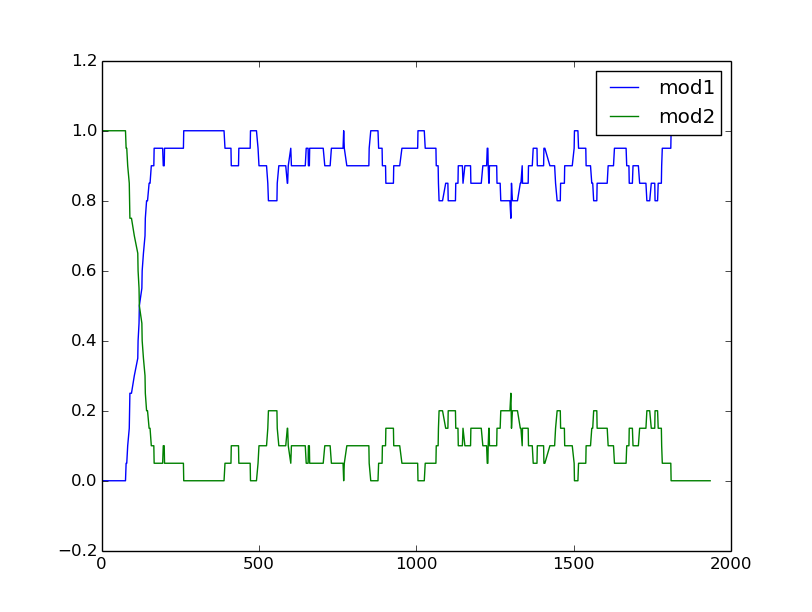
\includegraphics[width=8cm]{./include/choice_test_choices.png}
			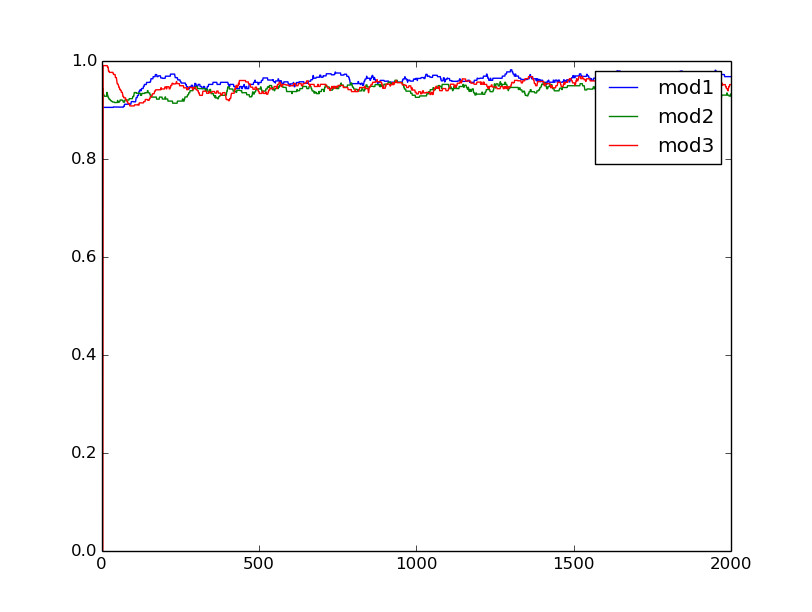
\includegraphics[width=8cm]{./include/choice_test_competences.png}
			%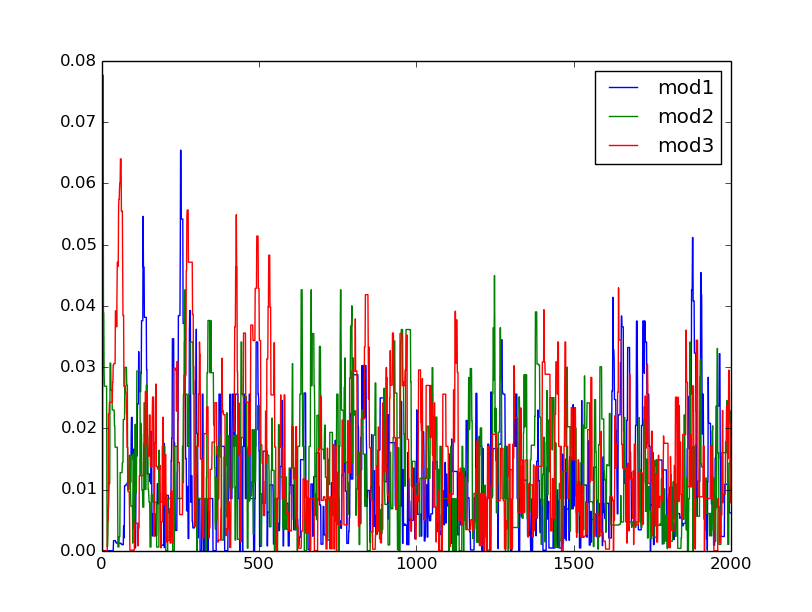
\includegraphics[width=8cm]{./include/choice_test_progresses.png}
			\caption{Progress on the 3 modules of a hierarchy with 2 choices of sub-modules for module 3. Left: Proportion of choices of module 3 (with a sliding window). Right: Competences (with a sliding window) of babbled points of each modules.}
			\label{fchoices}
		\end{figure}
		
	%
	
		
	\subsection{ZPDES}
	\label{zpdes}
	
		I've tested Benjamin's code of the ZPDES algorithm \cite{clement2014online} to choose which module to explore at each iterations.
		The algorithm has mainly 4 parameters:
		\begin{itemize}
			\item The rate $\alpha$ of integration of new information about average reward of bandits: $bandit\_value = (1 - \alpha) * old\_bandit\_value + \alpha * reward$. I used $\alpha = 0.5$.
			\item The activation threshold: if the mean (recent) competence of activated modules exceeds that threshold, then a new module will be activated. I used $0.5$.
			\item The deactivation threshold: if one module have its mean recent competence exceeding that threshold, it will be deactivated. I used $0.6$ here.
			\item A window size to compute the means of recent competences and progress: I used $20$ iterations.
		\end{itemize}
	
		See Fig. \ref{zpdesfig} for an exemple of execution of ZPDES in my setup. There are 3 modules with the same mathematical functions as forward models as in the previous section.
		We can see that module 1 gets deactivated early when its mean competence exceeds $0.6$.
		Module 3 only gets activated when the mean competence of modules 1 and 2 exceeds $0.5$ around $200$ iterations.
		
	
	
		\begin{figure}[H]
			\centering
			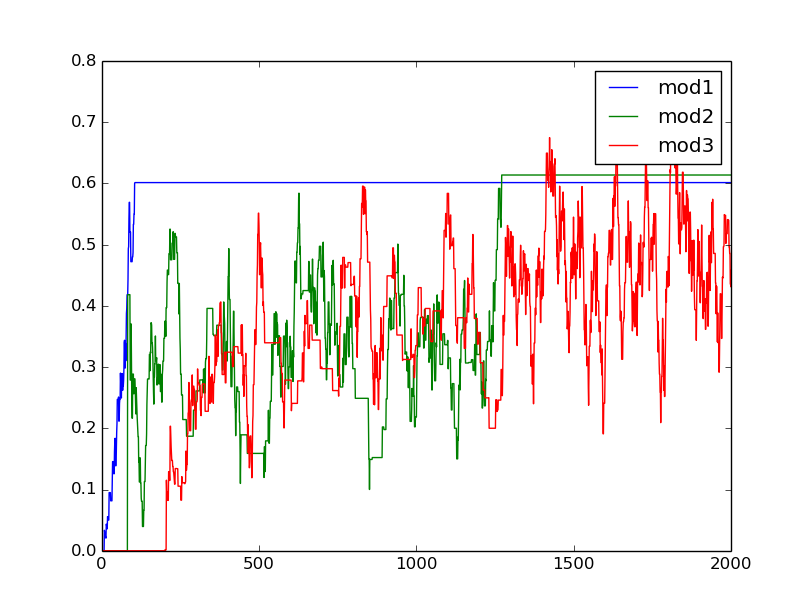
\includegraphics[width=8cm]{./include/ZPDES_competences.png}
			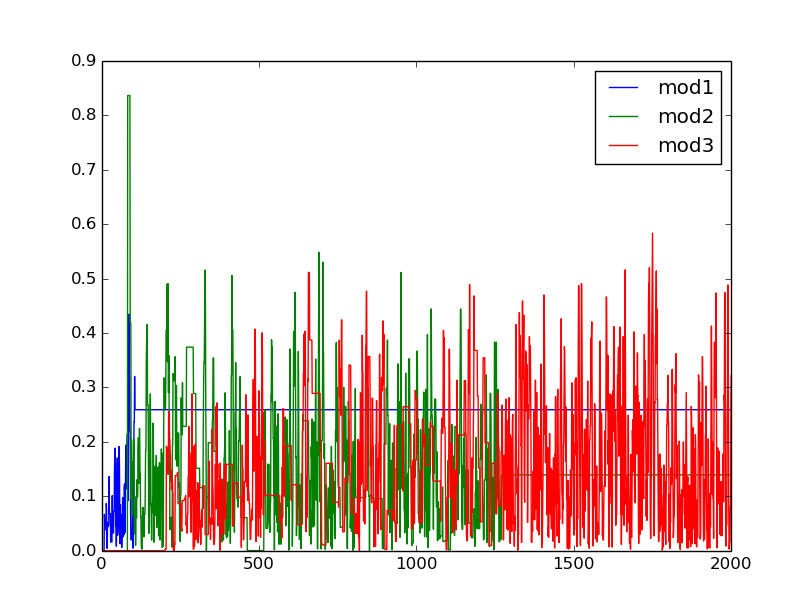
\includegraphics[width=8cm]{./include/ZPDES_progresses.png}
			\caption{Competences and progresses using ZPDES.}
			\label{zpdesfig}
		\end{figure}
	
		
		\paragraph{Remarks}
		
		The activation threshold allows to avoid spending useless trials on too complex tasks, provided the algorithm knows a sequence of modules sorted by increasing complexity or level in the hierarchy.		
		Also, the deactivation threshold allows to stop sampling tasks that are already mastered.
		However, if a task can't be mastered, for instance if a large part of the sensori space is not reachable (which is often the case), 
		then its competence might never exceed the deactivation threshold, which is not really a problem, and might even not exceed the activation threshold, at least if we use random goal babbling that might often 
		set unreachable goals. That could be a problem as only non progressing modules might be activated.
		One could lower the activation threshold but its benefit will be lower also.
		If SAGG-RIAC is used, the apparent competence will be the one on sampled points in progressing subregions of the tree, thus mostly in reachable parts, so that might not be an issue.
		
	%


%

\section{Summary}

	\paragraph{}%Résumé
	We have implemented and tested some of the described hierarchical exploration architectures in different environments (See Table \ref{recap}).
	
	
	\begin{table}[H]
		\centering
		\begin{tabular}{|l|l|l|c|}
		\hline
		\multicolumn{1}{|c|}{{\bf Problem}}                                                                  & \multicolumn{1}{c|}{{\bf Algorithm}}                                                        & \multicolumn{1}{c|}{{\bf Specificities}} & {\bf Implem. ?}   \\ \hline
		\multirow{4}{*}{\begin{tabular}[c]{@{}l@{}}Exploring autonomously \\ a fixed hierarchy\end{tabular}} & \multirow{2}{*}{\begin{tabular}[c]{@{}l@{}}Exploring models \\ in a hierarchy\end{tabular}} & Fixed learning cv                        & Yes                 \\ \cline{3-4} 
																											 &                                                                                             & Dynamic learning cv                      & Yes                 \\ \cline{2-4} 
																											 & \multirow{2}{*}{Top-Down Drive}                                                             & \begin{tabular}[c]{@{}l@{}}Models used by \\ max 1 model\end{tabular}               & Yes                 \\ \cline{3-4} 
																											 &                                                                                             & Other hierarchies                  & No                  \\ \hline
		\begin{tabular}[c]{@{}l@{}}Exploring tasks of \\increasing complexity\end{tabular}                                                                      & Creating modules   & Given M, S, O                            & Some                  \\ \hline
		\multicolumn{1}{|c|}{\multirow{3}{*}{Learning with Social Guidance}}                                 & \multirow{3}{*}{\begin{tabular}[c]{@{}l@{}}Integration of \\ Social Guidance\end{tabular}}  & Task-space level                         & \multirow{3}{*}{No} \\ \cline{3-3}
		\multicolumn{1}{|c|}{}                                                                               &                                                                                             & Model level                              &                     \\ \cline{3-3}
		\multicolumn{1}{|c|}{}                                                                               &                                                                                             & Hierarchy level                          &                     \\ \hline
		\end{tabular}
		\caption{Summary of developed algorithms}
		\label{recap}
	\end{table}
	
%

\section{Roadmap}
	
	%\paragraph{}%Missing Results = next steps	
	%In the learning algorithms tested, the hierarchy of models to learn is given to the agent as if it already knew the combinations of actions
	%to explore in order to learn the successive tasks.
	%This is a strong hypothesis as infants have first to discover what types of actions to combine to get a specific outcome.
	%The next step of this work is the implementation of the algorithm described in Section \ref{sec:increasing} that autonomously learns to progressively complexify 
	%the hierarchy of sensorimotor models.
	%Also, sensori contexts in models might simplify the use of sequencial actions and the design of sensori spaces.
	
	\paragraph{}%Future Studies
	The next important steps are to properly formulate, analyze and illustrate the different questions of this report, first in abstract settings before real experimental setups.
	The first question is how to explore a given, fixed hierarchy of tasks, and how the different algorithms behave (Section \ref{study1}).
	In those algorithms, the hierarchy of models to learn is given to the agent as if it already knew the combinations of actions to explore in order to learn the successive tasks.
	This is a strong hypothesis as infants have first to discover what types of actions to combine to get a specific outcome.	
	The second question is thus how and when to autonomously combine the previously learned actions in a relevant hierarchy of skills (Section \ref{study2}).	
	Then, we will study the integration of social guidance into those algorithms (Section \ref{study3}).
	
	\paragraph{}%Future Work:
	In future work, we also plan to make an experiment in which a robot has to autonomously 
	discover that sounds can influence a social peer (for example making him
	manipulate objects in the environment), using the extensions of our hierarchical exploration architectures that integrate social interaction (Section \ref{sec:social}). 
	Experiments will be conducted both through simulation of robotic environments and real robot
	experiments, in particular using the open-source humanoid platform Poppy.
	Then, we will work to allow for
	hierarchical reinforcement learning techniques in the model \cite{botvinick2012hierarchical}, in particular option
	theory \cite{sutton1999between}). 
	Also, we will study how techniques
	of multi-modal deep learning \cite{ngiam2011multimodal} can be used to select useful manifold in high-dimensional sensorimotor flows 
	(i.e. find useful lower dimensional abstractions of the flows) on which
	skill acquisition techniques can be applied.
	
%

\newpage

\section{Study 1: Exploration of a given hierarchy of skills}
\label{study1}

	\subsection{Introduction}

		Explain related work: \cite{vig, ugur2014, ugur2015}.
	
	%

	\subsection{Questions}

		\begin{itemize}
			\item Exploring in a structured hierarchy is more efficient than directly from $M$ to $S$.
			\item Which task should I explore now ?
			\item How to choose between different means to explore a given space ? 
			\item How can high-level tasks guide the exploration of lower-level ones ?
			\item How can the system cope with perturbations on some of the forward models ?		
		\end{itemize}

	%
	
	\subsection{Methods}
		
		\subsubsection{Algorithms}
		
			\paragraph{}
			Different module implementations (implemented):
			\begin{itemize}
				\item Motor Babbling,
				\item SAGG-Random.
			\end{itemize}
			
			\paragraph{}
			Different types of Sensorimotor models (implemented):
			\begin{itemize}
				\item NN or LWLR,
				\item NSLWLR to handle non stationary forward models (See Section \ref{NSLWLR}), or NSNN as NN plus a weighting by time.
			\end{itemize}
			
			\paragraph{}
			Different possibilities to handle exploration in the hierarchy (implemented):
			\begin{itemize}
				\item MAB on all modules (greedy, softmax),
				\item MAB biaised on lower modules (see Sec. \ref{NSLWLR}),
				\item ZPDES (see Sec. \ref{zpdes}).
			\end{itemize}
			
			\paragraph{}
			Different types of Top-Down Drive:
			\begin{itemize}
				\item Just add noise to motor command of each module (pb: interferes with competence and progress estimation)  (implemented),
				\item Exploration budget around goals asked by higher models (explonential in $levels^{n+1}$ so even $n=1$ is not feasible in general but maybe in practice)  (implemented),
				\item Exploration budget only for the modules one layer below the babbling module (not implemented).
				\item Balance self-computed interest with Top-Down interest (See Section \ref{tddkdtree}, not implemented).
			\end{itemize}
			
		
		%
		
		\subsubsection{Hierarchies}
		
		

			\begin{figure}[H] 
				\subfloat[]{
% H2
\begin{tikzpicture}[node distance=1cm,>=stealth',bend angle=45,auto]

	\tikzstyle{dom}   = [ellipse, thick, draw=black!75, fill=blue!20,  minimum height=4mm, minimum width=4mm]
	\tikzstyle{prim dom}   = [dom,  minimum height=5mm, minimum width=5mm,  fill=green!20]
	\tikzstyle{mod} = [rectangle, thick, draw=black!75, fill=black!20, minimum size=3mm]

	\begin{scope}
		\scriptsize
		\node [prim dom, label=below:$12$D] (pd1) {$Arm$};

		\node [mod, label=above:$Model_1$] (m1) [right of=pd1, xshift=-0.1cm] {$1$}
		edge [pre]                  (pd1);

		\node [dom, label=below:$9$D] (d1) [right of=m1] {$Hand$}
		edge [pre]                (m1);
		
		\node [mod] (m3) [right of=d1, xshift=-0.1cm,yshift=0.4cm] {$2$}
		edge [pre]                  (d1);
		
		\node [dom, label=below:$6$D] (d3) [right of=m3, xshift=-0.1cm,yshift=0.4cm] {$Stick_1$}
		edge [pre]                (m3);
		
		\node [mod] (m6) [right of=d1, xshift=-0.1cm,yshift=-0.4cm] {$5$}
		edge [pre]                  (d1);
		
		\node [dom, label=above:$6$D] (d6) [right of=m6, xshift=-0.1cm,yshift=-0.4cm] {$Stick_2$}
		edge [pre]                (m6);
		
		\node [mod] (m7) [right of=d6,yshift=0.2cm] {$6$}
		edge [pre]                  (d6);
		
		\node [mod] (m4) [right of=d3,yshift=-0.2cm] {$3$}
		edge [pre]                  (d3);
		
		\node [dom, label=below:$2$D] (d4) [right of=m4, xshift=-0.3cm,yshift=-0.6cm] {$Object$}
		edge [pre]                (m4)
		edge [pre]                (m7);
		
		\node [mod] (m5) [right of=d4] {$4$}
		edge [pre]                  (d4);
		
		\node [dom, label=below:$2$D] (d5) [right of=m5] {$Boxes$}
		edge [pre]                (m5);
		
		
	\end{scope}
	\begin{pgfonlayer}{background}
		\filldraw [line width=2mm,black!10]
		(d3.north  -| d5.east)  rectangle (d6.south  -| pd1.west);
	\end{pgfonlayer}
\end{tikzpicture}
}
				\subfloat[]{
% H2
\begin{tikzpicture}[node distance=1.cm,>=stealth',bend angle=45,auto]

	\tikzstyle{dom}   = [ellipse, thick, draw=black!75, fill=blue!20,  minimum height=5mm, minimum width=5mm]
	\tikzstyle{prim dom}   = [dom,  minimum height=5mm, minimum width=5mm,  fill=green!20]
	\tikzstyle{mod} = [rectangle, thick, draw=black!75, fill=black!20, minimum size=4mm]

	\begin{scope}
		\scriptsize
		\node [prim dom] (pd1) {$Arm_1$};
		
		\node [mod] (m1) [above of=pd1] {}
		edge [pre]                  (pd1);

		\node [dom] (d1) [above of=m1] {$Hand_1$}
		edge [pre]                (m1);
		
		\node [mod] (m2) [above of=d1, xshift=-1cm] {}
		edge [pre]                  (d1);
		
		\node [mod] (m3) [right of=m2, xshift=1cm] {}
		edge [pre]                  (d1);
		
		\node [dom] (d2) [above of=m2] {$Tool_1$}
		edge [pre]                (m2);
		
		\node [dom] (d3) [above of=m3] {$Tool_2$}
		edge [pre]                (m3);
		
		\node [mod] (m4) [above of=d2] {}
		edge [pre]                  (d2);
		
		\node [mod] (m5) [above of=d3] {}
		edge [pre]                  (d3);
		
		\node [dom] (d4) [above of=m4, xshift=1cm] {$Obj_1$}
		edge [pre]                (m4)
		edge [pre]                (m5);
		
		
	\end{scope}
	\begin{pgfonlayer}{background}
		\filldraw [line width=4mm,join=round,black!10]
		(d4.north  -| d3.east)  rectangle (pd1.south  -| d2.west);
	\end{pgfonlayer}
\end{tikzpicture}
}
				\subfloat[]{
% H3
\begin{tikzpicture}[node distance=1.cm,>=stealth',bend angle=45,auto]

	\tikzstyle{dom}   = [ellipse, thick, draw=black!75, fill=blue!20,  minimum height=5mm, minimum width=5mm]
	\tikzstyle{prim dom}   = [dom,  minimum height=5mm, minimum width=5mm,  fill=green!20]
	\tikzstyle{mod} = [rectangle, thick, draw=black!75, fill=black!20, minimum size=4mm]

	\begin{scope}
		\scriptsize
		\node [prim dom] (pd1) {$Arm_1$};
		
		\node [mod] (m1) [above of=pd1] {}
		edge [pre]                  (pd1);

		\node [dom] (d1) [above of=m1] {$Hand_1$}
		edge [pre]                (m1);
		
		\node [mod] (m2) [above of=d1, xshift=-1.6cm] {}
		edge [pre]                  (d1);
		
		\node [mod] (m3) [above of= d1, xshift=0.8cm] {}
		edge [pre]                  (d1);
		
		\node [dom] (d2) [above of=m2] {$Tool_1$}
		edge [pre]                (m2);
		
		\node [dom] (d3) [above of=m3] {$Tool_2$}
		edge [pre]                (m3);
		
		\node [mod] (m4) [above of=d2] {}
		edge [pre]                  (d2);
		
		\node [mod] (m5) [above of=d3, xshift=-0.8cm] {}
		edge [pre]                  (d3);
		
		\node [mod] (m6) [above of=d3, xshift=0.8cm] {}
		edge [pre]                  (d3);
		
		\node [dom] (d4) [above of=m4] {$Obj_1$}
		edge [pre]                (m4);
		
		\node [dom] (d5) [above of=m5] {$Obj_2$}
		edge [pre]                (m5);
		
		\node [dom] (d6) [above of=m6] {$Obj_3$}
		edge [pre]                (m6);
		
		
	\end{scope}
	\begin{pgfonlayer}{background}
		\filldraw [line width=4mm,join=round,black!10]
		(d4.north  -| d6.east)  rectangle (pd1.south  -| d2.west);
	\end{pgfonlayer}
\end{tikzpicture}
}
				\subfloat[]{
% H4
\begin{tikzpicture}[node distance=1.cm,>=stealth',bend angle=45,auto]

	\tikzstyle{dom}   = [ellipse, thick, draw=black!75, fill=blue!20,  minimum height=5mm, minimum width=5mm]
	\tikzstyle{prim dom}   = [dom,  minimum height=5mm, minimum width=5mm,  fill=green!20]
	\tikzstyle{mod} = [rectangle, thick, draw=black!75, fill=black!20, minimum size=4mm]

	\begin{scope}
		\scriptsize
		\node [prim dom] (pd1) {$Arm_1$};
		\node [prim dom] (pd2) [xshift=2cm] {$Arm_2$};
		
		\node [mod] (m1) [above of=pd1] {}
		edge [pre]                  (pd1);

		\node [dom] (d1) [above of=m1] {$Hand_1$}
		edge [pre]                (m1);
		
		\node [mod] (m2) [above of=pd2] {}
		edge [pre]                  (pd2);
		
		\node [dom] (d2) [above of=m2] {$Hand_2$}
		edge [pre]                (m2);
		
		\node [mod] (m3) [above of=d1] {}
		edge [pre]                  (d1);
		
		\node [dom] (d3) [above of=m3] {$Tool_1$}
		edge [pre]                (m3);
		
		\node [mod] (m4) [above of=d2] {}
		edge [pre]                  (d2);
		
		\node [dom] (d4) [above of=m4] {$Tool_2$}
		edge [pre]                (m4);
		
		\node [mod] (m5) [above of=d3, xshift=1cm] {}
		edge [pre]                  (d4)
		edge [pre]                  (d3);
		
		\node [dom] (d5) [above of=m5] {$Obj_1$}
		edge [pre]                (m5);
		
	\end{scope}
	\begin{pgfonlayer}{background}
		\filldraw [line width=4mm,join=round,black!10]
		(d5.north  -| d2.east)  rectangle (pd1.south  -| d1.west);
	\end{pgfonlayer}
\end{tikzpicture}
}
				\caption{Exemple of hierarchies.}
				\label{H}					
			\end{figure}
		%
		
		
		\subsubsection{Environment}
		
			\paragraph{}
			Different variables to test: motor and sensory dimensionalities, type of functions (linear, cosine, geometric arm, non-continuous interaction with objects), noise.
			
			\paragraph{Possible arm models:}
			\begin{itemize}
				\item $n$ DOFs 2D geometric arm
			\end{itemize}
			
			\paragraph{Possible tool models:}
			\begin{itemize}
				\item static piano
				\item stick 
			\end{itemize}
			
			\paragraph{Possible object models:}
			\begin{itemize}
				\item static object with features depending on the piano
				\item dynamic object
			\end{itemize}
			
		
		%
		

		\subsubsection{Experiments}

				% Experiment 1
				\paragraph{Experiment 1: Exploring in a structured hierarchy is more efficient than directly from $M$ to $S$.}				
				\begin{itemize}
					\item Idea: to compare our simplest algorithm (explore the module with higher progress) in a realistic setting (Hierarchy (a) of Fig. \ref{H}) to the control condition where a sensorimotor model is learned
							directly from the whole motor space $M$ to the whole sensori space $S$.
					
					\item Conditions: Hierarchy (a) vs $M \rightarrow S$, Motor Babbling vs SAGG-Random
					
					\item Features: MAB on all modules, NN, No TDD.
					
					\item Measures: exploration of intermediate spaces (hands, tools), exploration of top spaces (objects). Competence to reach random goals in reachable parts of intermediate and top spaces. 
							Statistics on multiple runs to see regularity/diversity in developmental trajectories.
				\end{itemize}
				
				% Experiment 2
				\paragraph{Experiment 2: Which task should I explore now ?}
				\begin{itemize}
					\item Idea: to compare the different possibilities to choose the module to explore in the hierarchy: maximizing the progress, maximizing with a bias towards lower-level modules, or use ZPDES,
							with the same hierarchy (a) of Fig. \ref{H}.
					
					\item Conditions: Random module, MAB on all modules, MAB with bias, ZPDES.
					
					\item Features: Hierarchy (a), SAGG-Random, NN, No TDD.
					
					\item Measures: exploration of intermediate spaces (hands, tools), exploration of top spaces (objects). Competence to reach random goals in reachable parts of intermediate and top spaces. 
							Statistics on multiple runs to see regularity/diversity in developmental trajectories.
				\end{itemize}
				
				% Experiment 3
				\paragraph{Experiment 3: How to choose between different means to explore a given space ?}
				\begin{itemize}
					\item Idea: to explain how we can choose between different means (e.g. different tools) using the one with the maximal competence, or maximal progress.
							We can use the hierarchy (b) of Fig. \ref{H}, in order to have 2 different tools to move the object.
					
					\item Conditions: maximize competence vs progress, noise on each tool, reachability (e.g. size) of each tool.
					
					\item Features: Hierarchy (b), MAB on all modules, SAGG-Random, NN, No TDD.
					
					\item Measures: exploration of intermediate spaces (hand, tools), exploration of top spaces (object). Competence to reach random goals in reachable parts of intermediate and top spaces. 
							Statistics on multiple runs to see regularity/diversity in developmental trajectories.
				\end{itemize}
				
				% Experiment 4
				\paragraph{Experiment 4: How can high-level tasks guide the exploration of lower-level ones ?}
				\begin{itemize}
					\item Idea: to compare different possibilities of Top-Down Guidance, with hierarchy (c) of Fig. \ref{H} in order to have TD guidance at different levels: 
							arm with one higher model, hand with 2 higher models, tool1 with one higher model, or tool2 with 2 higher models.
					
					\item Conditions: No TDD, Just add noise to motor command of each module (pb: interferes with competence estimation) 
							vs explore $n$ points and returns the best (warning: exponential)
							vs only one layer below the babbling module explores $n$ points.
					
					\item Features: Hierarchy (c), MAB on all modules with bias (or no bias?), SAGG-Random, NN.
					
					\item Measures: exploration of intermediate spaces (hands, tools), exploration of top spaces (objects). Competence to reach random goals in reachable parts of intermediate and top spaces. 
							Statistics on multiple runs to see regularity/diversity in developmental trajectories.
				\end{itemize}
				
				% Experiment 5
				\paragraph{Experiment 5: How can the system cope with perturbations on some of the forward models ?}
				\begin{itemize}
					\item Idea: to apply perturbations to one of the possible forward models, either blocking, shifting or randomizing one dimension. 
							We can use the hierarchy (d) of Fig. \ref{H} in order to see an adaptation at 2 levels: the use of one hand to use one tool, the use of both tools to move the object even if only one is perturbated.
					
					\item Conditions: No perturbations, which model is perturbated (arm, tool), type of perturbation (blocking, shifting, random).
					
					\item Features: Hierarchy (d), MAB on all modules, SAGG-Random, NN, best TDD.
					
					\item Measures: exploration of intermediate spaces (hands, tools) and top spaces (objects) before and after perturbations. 
							Competence to reach random goals in reachable parts of intermediate and top spaces before and after perturbations. 
							Statistics on multiple runs to see regularity/diversity in developmental trajectories.
				\end{itemize}

		%
	
	%
	
%


\section{Study 2: Curiosity-driven combination of skills}
\label{study2}


%


\section{Study 3: Socially-guided combination of skills}
\label{study3}

%


\bibliographystyle{apalike}
% argument is your BibTeX string definitions and bibliography database(s)
\small
\bibliography{./include/bibliography}

% that's all folks
\end{document}


